\documentclass[12pt]{book}
\usepackage[T1]{fontenc}
\usepackage{times}
\usepackage{listings}
\usepackage{graphicx}
\usepackage{xcolor}
\usepackage{url}
\usepackage{imakeidx}
\usepackage{booktabs}
\usepackage{array}
\usepackage{float}
\usepackage{url}
\usepackage{etoolbox}  % for showidx
\usepackage{fullpage}
\usepackage{soul}
\usepackage[utf8]{inputenc}
\usepackage{amsmath}

\usepackage{tikz}
\usetikzlibrary{shapes,arrows,positioning}
\usetikzlibrary{arrows.meta}
\usepackage{adjustbox}

\usepackage{hyperref}  % should be last
\definecolor{linkblue}{rgb}{0.05,0.25,0.65}
\hypersetup{
  pdfborder={0 0 0},
  colorlinks=true,
  linkcolor=linkblue,
  citecolor=linkblue,
  urlcolor=linkblue
}

\definecolor{codegreen}{rgb}{0,0.6,0}
\definecolor{codegray}{rgb}{0.5,0.5,0.5}
\definecolor{codepurple}{rgb}{0.58,0,0.82}

\lstdefinestyle{mystyle}{
    commentstyle=\color{codegreen},
    keywordstyle=\bfseries\color{magenta},
    stringstyle=\color{codepurple},
    basicstyle=\ttfamily\footnotesize,
    showstringspaces=false,
    xleftmargin=0.5cm
}
\lstset{style=mystyle}
\lstset{captionpos=b}

% Syntax highlighting for OctaC source: keywords (magenta, bold),
% line comments (green), no background shading.
\lstset{
    morekeywords={function, return, if, else, for, in, until, do, and, or,
                  not, is, true, false, i32, i64, f32, f64, bool, matrix,
                  vector, elseif, caseof, case, i16, default, break,
                  continue, f16, string},
    morecomment=[l]{//},
    morestring=[b]"
}

% Token name in a table cell: monospace, allowed to break after underscores.
\makeatletter
\def\tok@split#1_#2\@nil{#1\if\relax\detokenize{#2}\relax\else\_\allowbreak\tok@split#2\@nil\fi}
\newcommand{\tok}[1]{\texttt{\tok@split#1_\@nil}}
\makeatother

% Plain style for pseudocode listings (no keyword highlighting).
\lstdefinestyle{pseudocode}{
    keywordstyle=\relax,
    stringstyle=\relax
}

% One space after periods
\frenchspacing

% Do not stretch vertical space to fill pages, so unbreakable blocks
% (tables, listings) never leave large gaps around them.
\raggedbottom

\hypersetup{pdfauthor={Syed Taha, Muhammad Usman},
            pdftitle={OctaC: A Language Specification},}

\lstset{basicstyle=\small\ttfamily}
\lstset{escapeinside={(*@}{@*)}}
\lstset{xleftmargin=5.0ex}

\newcommand{\github}{https://github.com/mit-pdos/xv6-riscv/blob/riscv/}

\newcommand{\fileref}[1]{\small{\textcolor{red}{(#1)}}}
\newcommand{\lineref}[2]{\small{\textcolor{red}{(#1:#2)}}}
\newcommand{\linerefs}[3]{\small{\textcolor{red}{(#1:#2-#3)}}}

\newcommand{\showfileref}[2]{\href{\github/#1}{\small{(\textcolor{blue}{#2})}}}
\newcommand{\showlineref}[3]{\href{\github/#1\#L#2}{\small{(\textcolor{blue}{#3})}}}
\newcommand{\showlinerefs}[5]{\href{\github/#1\#L#2-L#3}{\small\textcolor{blue}{(#4-#5)}}}

\newcommand{\indextext}[1]{\textit{#1}\index{#1}}
\newcommand{\indextextx}[1]{{#1}\index{#1}}
\newcommand{\indexcode}[1]{\lstinline{#1}\index{#1@\lstinline{#1}}}

%% editing markup
\newcommand{\insertnote}[3]{\noindent\textcolor{#1}{\textbf{#2:} #3}}
\newcommand{\note}[1]{\insertnote{blue}{NOTE}{#1}}

% ------------------------------------------------------------
% Inline code styling
% ------------------------------------------------------------
\usepackage[most]{tcolorbox}

\tcbset{
    myinlinecode/.style={
        enhanced,
        boxsep=0.3mm,
        left=0.5mm,
        right=0.5mm,
        top=0.5mm,
        bottom=0.5mm,
        colback=gray!20, % background color
        colframe=gray!20, % optional border color
        arc=1mm,          % rounded corners
        boxrule=0pt,    % border thickness
        box align=base,   % aligns nicely with text
        before skip=0pt,
        after skip=0pt,
        fontupper=\ttfamily % monospace font
    }
}

% Command for easier usage
\newtcbox{\code}{myinlinecode, tcbox raise=0pt, box align=base, on line}

\title{\textbf{OctaC: A Language Specification}\\[0.3em]
\large Designing a Hybrid Language for Numerical and Matrix Computation}
\author{Syed Taha \and Muhammad Usman}

\makeindex

\begin{document}

\maketitle

{\hypersetup{linkcolor=black}\tableofcontents}

\chapter*{Foreword and acknowledgments}

This text details the design of OctaC, a statically typed, C-structured
language for numerical and matrix computation, along with the compiler
built to implement it. The chapters assembled here document the language
specification and the design decisions made along the way.

We acknowledge the support and guidance of our supervisor, Miss Sadaf Alvi,
whose feedback helped shape the project goals and technical approach.

The work was carried out by Syed Taha and Muhammad Usman. It was completed
as part of the Compiler Construction course at our university. For
questions, bug reports, or further information about the implementation,
please contact Syed Taha at s.taha.29208@khi.iba.edu.pk.

\addcontentsline{toc}{chapter}{Foreword and acknowledgments}

\chapter*{Preface}

OctaC is a statically typed, C-structured language for numerical and
matrix computation. Dynamically typed languages like Octave
\cite{octave-manual} let a programmer multiply two matrices of incompatible
shapes without complaint until the operation actually runs. A statically
typed language can catch that mistake before a single instruction executes,
but only if the compiler is taught to treat shape, not just type, as a
property of a value that can be checked at compile time. OctaC brings that
discipline to a C-structured surface syntax, with scalar types (\code{i16},
\code{i32}, \code{i64}, \code{f16}, \code{f32}, \code{f64}, \code{bool})
alongside matrix and vector types parameterized by their element type
(\code{matrix<i32>}, \code{vector<f32>}).

This is a living book. It begins with an introduction to OctaC and its
lexical analysis, and is meant to grow chapter by chapter as the compiler is
built over time: the formal grammar, the parser, the semantic analysis pass,
and code generation will each be added as their own chapter once they exist.
Chapter~1 introduces the language as it currently stands, and Chapter~2
covers its lexer.

This book prioritizes clarity and feasibility over completeness. Where we
simplify (omit a feature, restrict a rule, choose one semantic
over another), we try to say so explicitly rather than let the omission
speak for itself.

We hope it serves as both a reference for the finished language and an
honest record of the decisions, and trade-offs, behind it.

\begin{lstlisting}[breaklines=true]
function main() -> i32 {
    printf("Hello, world!\n");
    return 0;
}
\end{lstlisting}

\addcontentsline{toc}{chapter}{Preface}

%  Part 1: Language Design
\part{Language Design}
% p1-chp01-introduction.tex

\chapter{Introduction}
\label{chp:introduction}

OctaC is a small, statically typed language for numerical and matrix
computation. Its purpose is to make numerical scripts, matrix operations,
and iterative computations easy to read and easy to write, without giving
up static typing.

This chapter introduces the language at a high level: the motivation behind
it, the languages it draws on, the features it offers, and the shape of its
syntax through a set of sample programs. The precise definition of its
tokens, and the lexer that recognizes them, follows in
Chapter~\ref{chp:lexer}.

\section{Motivation}
\label{sec:motivation}

Languages built for matrix work, such as Octave and MATLAB, make matrices
and vectors easy to write, but they are dynamically typed
\cite{octave-manual,matlab-docs}. A program that multiplies two matrices of
incompatible shapes is accepted as written and fails only when the operation
runs. Languages such as C and C++ check types before a program runs, but
treat matrices as library structures or nested arrays, and leave the
arithmetic to hand written loops \cite{kernighan1988c,stroustrup2013cpp}.

OctaC sits between the two. Matrices and vectors are built in types, and
their arithmetic is part of the language. This requires the semantic
analysis phase to track shape alongside type: operations on statically known
shapes are checked at compile time, while operations on shapes that depend
on a function parameter, a return value, or a loop built matrix are checked
at runtime.

\section{Design Influences}

OctaC is a hybrid rather than a subset of a single language. Each part of
its design comes from the language that handles it best:

\begin{itemize}
    \item \textbf{Octave and MATLAB} for matrix and vector arithmetic
    \cite{octave-manual,matlab-docs}.
    \item \textbf{C and C++} for block structure and statement syntax
    \cite{kernighan1988c,stroustrup2013cpp}.
    \item \textbf{Rust and Zig} for explicit sized primitive types
    \cite{rust-book,zig-reference}.
    \item \textbf{Python} for range based and \code{for...in} iteration, and
    for English word logical operators (\code{and}, \code{or}, and so on)
    \cite{python-reference}.
\end{itemize}

\section{Features}

\noindent\textbf{Native matrix and vector types.} Matrices and vectors are
built in types, not library structures. Operators are split between true
matrix arithmetic (\code{*} for multiplication, \code{'} for transpose) and
element wise arithmetic (\code{.+}, \code{.*}, and related operators), so
the operation being performed is visible at the point of use.

Beyond this, OctaC supports:

\begin{itemize}
    \item Explicit sized variable declarations (\code{i32}, \code{f32},
    \code{bool}, \code{matrix<i32>}, \code{matrix<f32>}, and related types)
    \item Block scoping with shadowing in nested blocks
    \item Scalar, matrix, and element wise operators
    \item Assignment, including compound forms (\code{+=}, \code{*=})
    \item Conditionals: \code{if} / \code{else if} / \code{else}, using
    English word logic (\code{and}, \code{or}, \code{not}, \code{is})
    \item Loops: range based \code{for}, \code{for...in}, \code{until},
    \code{do...until}
    \item Functions with typed parameters and an explicit return type
    \item Matrix and vector literals and indexing
\end{itemize}

\section{Sample Programs}

The following programs show the syntax of OctaC in use. Each one is a
complete program, followed by a walkthrough of the constructs it introduces.
Later programs build on what earlier ones explain, so they are best read in
order.

A few things are common to all of them. A program is made of functions, and
execution starts in the function named \code{main}, which returns an
\code{i32}. Statements end with a semicolon, and blocks are delimited by
braces, as in C. A comment starts with \code{//} and runs to the end of the
line. Output is written with \code{printf}, whose format string follows the
one in C \cite{kernighan1988c}: \code{\%d} prints an integer and \code{\%.2f}
prints a floating point number with two digits after the point. OctaC adds
\code{\%m}, which prints a matrix or a vector.

\subsection{Sum of Squares}

The first program adds up the squares of the numbers from 1 to 5. It shows the
basic building blocks of the language: a function, a typed variable, a loop,
and output.

\begin{lstlisting}
function main() -> i32 {
    i32 sum = 0;
    for (i32 i = 1...5) {
        sum += i * i;
    }
    printf("Sum: %d\n", sum);
    return 0;
}
\end{lstlisting}

The header \code{function main() -> i32} declares a function. The empty
parentheses are its parameter list, and the arrow introduces its return type,
so the type of the result is always written after the parameters. Inside the
body, \code{i32 sum = 0;} declares a variable. Every declaration in OctaC
follows the same order: the type first, then the name, then the initial value.

The loop \code{for (i32 i = 1...5)} is a range loop. It declares its own
counter, \code{i}, and counts it from 1 up to and including 5, using the range
operator \code{...}. Each pass adds \code{i * i} to the running total with the
compound assignment \code{+=}, so the program prints \code{Sum: 55}.

\subsection{Matrix Multiplication}

The second program shows the feature the language is built around, which is
that matrices are a native type rather than something a library provides.

\begin{lstlisting}
function main() -> i32 {
    matrix<i32> A = [[1, 2], [3, 4]];
    matrix<i32> B = [[5, 6], [7, 8]];
    matrix<i32> C = A * B;
    printf("A * B:\n%m\n", C);
    return 0;
}
\end{lstlisting}

The type \code{matrix<i32>} is a matrix whose elements are \code{i32}. A
matrix literal is written as a list of rows, and each row is itself a list in
brackets, so \code{[[1, 2], [3, 4]]} is a matrix with two rows and two
columns. Because \code{A} and \code{B} are initialized with literals at the
point of declaration, their shapes are known, and the declaration does not
need to state them.

The expression \code{A * B} is true matrix multiplication. Its value is
stored in \code{C}, and is the matrix \code{[[19, 22], [43, 50]]}. This
is different from element wise multiplication, which has an operator of its own.
The expression \code{A .* B} would multiply the entries position by position,
and would give the matrix \code{[[5, 12], [21, 32]]}. Because the shapes
of \code{A} and \code{B} are known, the compiler can check that they are
compatible for multiplication before the program runs. The format specifier
\code{\%m} prints the result.

\subsection{Matrix-Vector Product}

The third program combines the two native types by multiplying a $2 \times 3$
matrix by a vector of 3 elements ($A\mathbf{x}$), which produces a vector of
2 elements.

\begin{lstlisting}
function main() -> i32 {
    matrix<f32> A = [
        [1.0, 2.0, 3.0],
        [4.0, 5.0, 6.0]
    ];
    vector<f32> x = [2.0, 1.0, 0.0];

    // Linear transformation Ax -> 2x1 vector
    vector<f32> y = A * x;

    printf("Result y = Ax: %m\n", y);
    return 0;
}
\end{lstlisting}

Here \code{vector<f32>} is a vector of \code{f32} elements, written as a
single bracketed list. The matrix literal is spread over several lines, since
whitespace is not significant, and the comment marks what the multiplication
computes. The shape of the result follows the same rule as for two matrices:
it has as many rows as the left operand, and the multiplication is only valid
when the number of columns of \code{A} matches the number of elements of
\code{x}. Here both are 3, so \code{y} has 2 elements, namely
\code{[4.0, 13.0]}.

\subsection{Iterative Convergence}

The fourth program introduces conditions and the \code{until} loop. It halves a
value until it drops below a threshold, or until a step limit is reached.

\begin{lstlisting}
function main() -> i32 {
    f32 val = 100.0;
    i32 steps = 0;
    until (val < 1.0 or steps is 20) {
        val /= 2.0;
        steps += 1;
    }
    printf("Converged in %d steps.", steps);
    return 0;
}
\end{lstlisting}

An \code{until} loop runs as long as its condition is false, and stops as soon
as the condition becomes true. It is the reverse of the \code{while} loop of
C: the condition states when to stop rather than when to continue. The
condition here combines two tests. The comparison \code{val < 1.0} keeps its
symbolic form, while equality is written with the word \code{is}, and the two
tests are joined by \code{or}. The loop therefore ends when the value has
fallen below 1, or after 20 passes, whichever comes first. The second test
guards against a loop that would otherwise never end.

The body uses the compound assignments \code{/=} and \code{+=}. The value is
halved seven times before it falls below 1, so the program prints
\code{Converged in 7 steps.}

\subsection{Input Validation}

The fifth program reads a value from the user and keeps asking until it is
valid. It shows the \code{do...until} loop, which always runs at least once.

\begin{lstlisting}
function main() -> i32 {
    f32 val = 0.0;
    do {
        printf("Enter a nonzero val: ");
        val = input();
    } until (val is not 0.0);
    printf("Accepted: %.2f\n", val);
    return 0;
}
\end{lstlisting}

In a \code{do...until} loop the body comes first and the condition is checked
afterwards, so the prompt is always shown at least once. The function
\code{input()} reads a value from the user. The condition uses \code{is not},
the word form of inequality, so the loop repeats until the value entered is not
zero. The variable is given the initial value \code{0.0} so that it holds a
defined value before the first read.

\subsection{GPU-Accelerated Matrix Operations}

The last program shows two more parts of the type system: precision and
statically declared sizes.

\begin{lstlisting}
function main() -> i32 {
    // Statically sized matrix
    matrix<f16, 1024, 1024> A = identity();

    // can auto-infer size
    matrix<f16> B = A * 2.5;

    matrix<f16, 1024, 1024> C = A * B;

    return 0;
}
\end{lstlisting}

The element type \code{f16} is a half precision floating point number. In the
declaration of \code{A}, the dimensions are written as part of the type, so
this is a matrix of 1024 by 1024 elements. The matrix \code{B} is declared
without dimensions, because they can be inferred from the expression that
initializes it: multiplying \code{A} by the scalar \code{2.5} scales every
element and keeps the shape.

The last line multiplies two large matrices. Operations on matrices of this
size are meant to be offloaded to a GPU automatically when one is available,
without the program containing any GPU specific code.

\section{Looking Ahead}

The programs above show the surface of OctaC: typed declarations, native
matrices and vectors, two families of arithmetic operators, English word
conditions, and four kinds of loops. What they leave open is how a program
like these becomes something a machine can run. That is the job of the
compiler, which works in phases \cite{aho2006compilers}.

The first phase, lexical analysis, reads the program as a stream of
characters and splits it into tokens such as \code{for}, \code{i32}, \code{1},
and \code{...}. Chapter~\ref{chp:lexer} defines these tokens precisely and
shows how the lexer recognizes them. The later phases give the tokens a
structure and a meaning, and they are where the shape checking described in
Section~\ref{sec:motivation} takes place. They will be added to this book as
they are built.

% p1-chp02-lexer.tex

\chapter{Lexical Analysis and the Lexer}
\label{chp:lexer}

The lexical analyzer, or lexer, is the first phase of the compiler. It reads
the source program as a stream of characters and groups them into tokens,
the units that the parser works with \cite{aho2006compilers}. This chapter
defines the full token specification of OctaC, the deterministic finite
automata that recognize those tokens
\cite{aho2006compilers,hopcroft2006automata}, and the algorithm the lexer
uses to drive them. The source code of the lexer is available at:
\url{https://github.com/Octa-C/lexer}

\section{Token Specification}

This section lists the complete token set for the lexical analyzer, in
Table~\ref{tab:token-set}. Every token belongs to a category, and some are
divided further into a subcategory. The loop keywords \code{for}, \code{do},
\code{until}, and \code{continue}, for example, belong to the Keyword category
and the Loops subcategory. The Token column gives the token as it is written
in the source, or a descriptive name where one token covers several lexemes.
The Values column is filled only for those tokens that match more than one
lexeme, or a pattern, such as the scalar datatypes or the integer literals,
and lists the lexemes or the regular expression they match. The last column
gives the generated name of the token, built from its category, subcategory,
and token in the form \code{CATEGORY\_SUBCATEGORY\_TOKEN}, which is the name
used to identify the token from here on.

The logical and equality operators are written as English words, so they are
listed among the keywords rather than the operators. The two compiler tokens,
EOF and Error, do not correspond to any source text and are produced by the
lexer itself.

\begin{table}[tbp]
\centering
\fontsize{6.2}{7.2}\selectfont
\renewcommand{\arraystretch}{1.1}
\setlength{\tabcolsep}{2pt}
\begin{tabular}{@{}ll@{\hspace{6pt}}ll@{\hspace{6pt}}l@{}}
\toprule
\textbf{Category} & \textbf{Subcategory} & \textbf{Token} & \textbf{Values} & \textbf{Generated token} \\
\midrule
Keyword & Loops & \texttt{for} &  & \tok{KW_LOOPS_FOR} \\
Keyword & Loops & \texttt{do} &  & \tok{KW_LOOPS_DO} \\
Keyword & Loops & \texttt{until} &  & \tok{KW_LOOPS_UNTIL} \\
Keyword & Loops & \texttt{continue} &  & \tok{KW_LOOPS_CONTINUE} \\
Keyword & Function & \texttt{function} &  & \tok{KW_FUNC_FUNCTION} \\
Keyword & Function & \texttt{return} &  & \tok{KW_FUNC_RETURN} \\
Keyword & Conditional & \texttt{if} &  & \tok{KW_CONDITIONAL_IF} \\
Keyword & Conditional & \texttt{else} &  & \tok{KW_CONDITIONAL_ELSE} \\
Keyword & Conditional & \texttt{elseif} &  & \tok{KW_CONDITIONAL_ELSEIF} \\
Keyword & Conditional & \texttt{caseof} &  & \tok{KW_CONDITIONAL_CASEOF} \\
Keyword & Conditional & \texttt{case} &  & \tok{KW_CONDITIONAL_CASE} \\
Keyword & Conditional & \texttt{default} &  & \tok{KW_CONDITIONAL_DEFAULT} \\
Keyword & Word-based Logic/Rel Ops & \texttt{and} &  & \tok{KW_WORDBASED_LOGICREL_OPS_AND} \\
Keyword & Word-based Logic/Rel Ops & \texttt{or} &  & \tok{KW_WORDBASED_LOGICREL_OPS_OR} \\
Keyword & Word-based Logic/Rel Ops & \texttt{not} &  & \tok{KW_WORDBASED_LOGICREL_OPS_NOT} \\
Keyword & Word-based Logic/Rel Ops & \texttt{is} &  & \tok{KW_WORDBASED_LOGICREL_OPS_IS} \\
Keyword & Word-based Logic/Rel Ops & \texttt{in} &  & \tok{KW_WORDBASED_LOGICREL_OPS_IN} \\
Keyword & Misc & \texttt{break} &  & \tok{KW_MISC_BREAK} \\
\midrule
Datatype &  & Scalar & \texttt{i64}, \texttt{i32}, \texttt{i16}, \texttt{f64}, \texttt{f32}, \texttt{f16}, \texttt{bool} & \tok{DT_SCALAR} \\
Datatype &  & \texttt{vector} &  & \tok{DT_VECTOR} \\
Datatype &  & \texttt{matrix} &  & \tok{DT_MATRIX} \\
Datatype &  & \texttt{string} &  & \tok{DT_STRING} \\
\midrule
Punctuation &  & \texttt{\{} &  & \tok{PUNCTUATION_LBRACE} \\
Punctuation &  & \texttt{\}} &  & \tok{PUNCTUATION_RBRACE} \\
Punctuation &  & \texttt{(} &  & \tok{PUNCTUATION_LPAREN} \\
Punctuation &  & \texttt{)} &  & \tok{PUNCTUATION_RPAREN} \\
Punctuation &  & \texttt{[} &  & \tok{PUNCTUATION_LBRACKET} \\
Punctuation &  & \texttt{]} &  & \tok{PUNCTUATION_RBRACKET} \\
Punctuation &  & \texttt{;} &  & \tok{PUNCTUATION_SEMICOLON} \\
Punctuation &  & \texttt{->} &  & \tok{PUNCTUATION_ARROW} \\
Punctuation &  & \texttt{,} &  & \tok{PUNCTUATION_COMMA} \\
Punctuation &  & \texttt{...} &  & \tok{PUNCTUATION_ELLIPSIS} \\
Punctuation &  & \texttt{:} &  & \tok{PUNCTUATION_COLON} \\
\midrule
Operators & Standard & \texttt{+-} & \texttt{+}, \texttt{-} & \tok{OPERATORS_STANDARD_PLUSMINUS} \\
Operators & Standard & \texttt{* / \%} & \texttt{*}, \texttt{/}, \texttt{\%} & \tok{OPERATORS_STANDARD_STAR_SLASH_MOD} \\
Operators & Matrix & \texttt{'} &  & \tok{OPERATORS_MATRIX_TRANSPOSE} \\
Operators & Matrix & \texttt{.*} &  & \tok{OPERATORS_MATRIX_DOT_STAR} \\
Operators & Matrix & \texttt{./} &  & \tok{OPERATORS_MATRIX_DOT_SLASH} \\
Operators & Relational and Comparison Ops & \texttt{<} &  & \tok{OPERATORS_RELATIONAL_AND_COMPARISON_OPS_LESS} \\
Operators & Relational and Comparison Ops & \texttt{>} &  & \tok{OPERATORS_RELATIONAL_AND_COMPARISON_OPS_GREATER} \\
Operators & Relational and Comparison Ops & \texttt{<=} &  & \tok{OPERATORS_RELATIONAL_AND_COMPARISON_OPS_LESS_EQ} \\
Operators & Relational and Comparison Ops & \texttt{>=} &  & \tok{OPERATORS_RELATIONAL_AND_COMPARISON_OPS_GREATER_EQ} \\
Operators & Assignment &  & \texttt{=}, \texttt{+=}, \texttt{-=}, \texttt{*=}, \texttt{/=} & \tok{OPERATORS_ASSIGNMENT} \\
\midrule
Identifier &  & identifier & \texttt{[a-zA-Z][a-zA-Z0-9\_]*} & \tok{IDENTIFIER} \\
\midrule
Constants &  & bool constant & \texttt{1}, \texttt{0} & \tok{CONSTANTS_BOOL_CONSTANT} \\
Constants &  & int literal & \texttt{[0-9]+} & \tok{CONSTANTS_INT_LITERAL} \\
Constants &  & float literal & \begin{tabular}[t]{@{}l@{}}\texttt{[0-9]+\textbackslash .[0-9]+}\\ \texttt{[0-9]+(\textbackslash .[0-9]+)?[eE][+-]?[0-9]+}\end{tabular} & \tok{CONSTANTS_FLOAT_LITERAL} \\
Constants &  & string literal & \texttt{"[\textasciicircum "\textbackslash n]*"} & \tok{CONSTANTS_STRING_LITERAL} \\
\midrule
Compiler &  & EOF &  & \tok{COMPILER_EOF} \\
Compiler &  & Error &  & \tok{COMPILER_ERROR} \\
\bottomrule
\end{tabular}
\caption{The OctaC token set.}
\label{tab:token-set}
\end{table}

\section{Deterministic Finite Automata}

The lexer recognizes every token of OctaC with a single deterministic finite
automaton, driven by a transition table
\cite{aho2006compilers,hopcroft2006automata}. The automaton only recognizes
the shape of a lexeme, such as a word, a number, or an operator. Which token
that lexeme becomes is decided afterwards by a lookup, described in
Section~\ref{sec:lexer-algorithm}. This keeps the automaton small: reserved
words do not need a path of their own, because they have the same shape as
identifiers. The subsections below describe the part of the automaton that
handles each class of tokens, and each has its own diagram. The last
subsection merges them into the one automaton that the lexer runs.

\subsection{Character Classes}

The automaton does not look at individual characters. Each input byte is first
mapped to one of 17 character classes, and the transition table has one
column per class. The letters \code{e} and \code{E} have a class of their own
because they can begin the exponent of a number, while everywhere else they
behave like any other letter. Table~\ref{tab:classes} lists the classes.

\begin{table}[H]
\centering
\footnotesize
\begin{tabular}{@{}ll@{}}
\code{LETTER} & \code{A-D} \code{F-Z} \code{a-d} \code{f-z} \\
\code{EXP} & \code{E} \code{e} \\
\code{DIGIT} & \code{0-9} \\
\code{\_} & \code{\_} \\
\code{WS} & \code{\symbol{92}t} \code{\symbol{92}v} \code{\symbol{92}f} \code{\symbol{92}r} \code{space} \\
\code{NL} & \code{\symbol{92}n} \\
\code{QUOTE} & \code{\symbol{34}} \\
\code{DOT} & \code{.} \\
\code{PLUS} & \code{+} \\
\code{MINUS} & \code{-} \\
\code{STAR} & \code{*} \\
\code{SLASH} & \code{/} \\
\code{LT} & \code{<} \\
\code{GT} & \code{>} \\
\code{EQ} & \code{=} \\
\code{SIMPLE} & \code{\%} \code{\textquotesingle{}} \code{(} \code{)} \code{,} \code{:} \code{;} \code{[} \code{]} \code{\symbol{123}} \code{\symbol{125}} \\
\code{OTHER} & any other character \\
\end{tabular}
\caption{Character classes of the lexer.}
\label{tab:classes}
\end{table}

\subsection{States}

The automaton has 19 states, listed in Table~\ref{tab:dfa-states}. A state is
accepting when it has an action, which says what the lexeme read so far
produces. States without an action are only stepping stones towards a longer
lexeme.

\begin{table}[H]
\centering
\footnotesize
\renewcommand{\arraystretch}{1.1}
\begin{tabular}{@{}l>{\raggedright\arraybackslash}p{190pt}>{\raggedright\arraybackslash}p{130pt}@{}}
\toprule
\textbf{State} & \textbf{Reached after reading} & \textbf{Action} \\
\midrule
\code{DEAD} & no valid continuation exists (error state) & none \\
\code{START} & nothing yet & none \\
\code{IDENT} & \code{[a-zA-Z][a-zA-Z0-9\_]*} & keyword lookup, else identifier \\
\code{INT} & \code{[0-9]+} & integer literal \\
\code{INT\_DOT} & an integer and a dot, such as \code{12.} & none \\
\code{FLOAT} & \code{[0-9]+\textbackslash .[0-9]+} & float literal \\
\code{EXP} & a number and \code{e} or \code{E} & none \\
\code{EXP\_SIGN} & a number, \code{e} or \code{E}, and a sign & none \\
\code{FLOAT\_EXP} & a number with a complete exponent & float literal \\
\code{OP\_DONE} & an operator or punctuator that cannot be extended, such as \code{\{}, \code{->}, \code{<=}, \code{...}, \code{.*} or \code{=} & operator lookup \\
\code{MINUS} & \code{-}, which may extend to \code{->} or \code{-=} & operator lookup \\
\code{OP\_EQ} & \code{<}, \code{>}, \code{+} or \code{*}, which may extend with \code{=} & operator lookup \\
\code{SLASH} & \code{/}, which may extend to \code{/=} or begin a comment & operator lookup \\
\code{COMMENT} & \code{//} and the rest of the line & skip \\
\code{DOT} & \code{.}, waiting for \code{*}, \code{/} or another \code{.} & none \\
\code{DOT\_DOT} & \code{..}, waiting for a third \code{.} & none \\
\code{STR\_BODY} & an opening quote and the text after it & none \\
\code{STR\_END} & a complete string literal & string literal \\
\code{WS} & a run of whitespace & skip \\
\bottomrule
\end{tabular}
\caption{States of the lexer DFA.}
\label{tab:dfa-states}
\end{table}

\subsection{Identifiers, Keywords, and Type Names}

An identifier has the pattern \code{[a-zA-Z][a-zA-Z0-9\_]*}: a letter followed
by any number of letters, digits and underscores. The DFA has one accepting
state, \code{IDENT}, and it emits \textless IDENTIFIER, value\textgreater.
Keywords and type names have the same shape, so the DFA reads them as
identifiers as well. After the DFA accepts, the lexer looks the lexeme up in
Table~\ref{tab:lookup}. A lexeme that is in the table gets the keyword or type
token given there in place of \textless IDENTIFIER, value\textgreater.

An underscore cannot start an identifier, so it has no transition out of
the start state and is reported as a lexical error.

\begin{figure}[H]
\centering
\begin{adjustbox}{max width=\linewidth,max height=0.3\textheight}
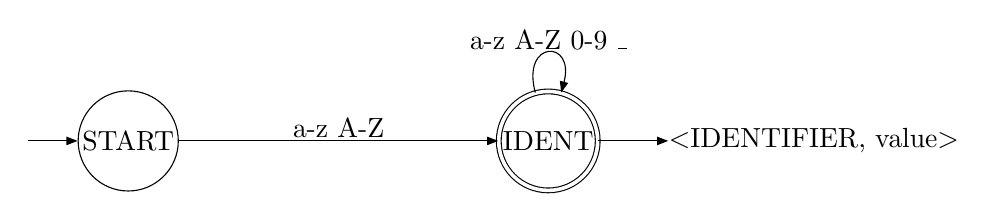
\begin{tikzpicture}[x=1in,y=1in,line width=0.4pt]
\node[draw,circle,fill=white,inner sep=1pt,minimum size=0.42in] (START) at (0.9,0.7) {START};
\node[draw,circle,fill=white,inner sep=1pt,minimum size=0.42in,double,double distance=1.3pt] (IDENT) at (3.0,0.7) {IDENT};
\draw[-{Triangle[length=4bp,width=3bp]}] (0.4,0.7) -- (START);
\node[inner sep=0pt,align=left,anchor=west] (IDENT-out) at (3.6,0.7) {\textless{}IDENTIFIER, value\textgreater{}};
\draw[-{Triangle[length=4bp,width=3bp]}] (START) to[bend left=0] node[pos=0.5,above,inner sep=1pt,align=center] {\code{a-z} \code{A-Z}} (IDENT);
\path[-{Triangle[length=4bp,width=3bp]}] (IDENT) edge[loop above,min distance=7mm] node[above,inner sep=1pt,align=center] {\code{a-z} \code{A-Z} \code{0-9} \code{\_}} (IDENT);
\draw[-{Triangle[length=4bp,width=3bp]}] (IDENT) to[bend left=0] (IDENT-out.west);
\end{tikzpicture}
\end{adjustbox}
\caption{DFA for identifiers, keywords, and type names.}
\label{fig:dfa-ident}
\end{figure}

\begin{table}[H]
\centering
\footnotesize
\begin{tabular}{@{}ll@{}}
\code{for} & \textless{}KW\_LOOPS\_FOR,\textgreater{} \\
\code{do} & \textless{}KW\_LOOPS\_DO,\textgreater{} \\
\code{until} & \textless{}KW\_LOOPS\_UNTIL,\textgreater{} \\
\code{continue} & \textless{}KW\_LOOPS\_CONTINUE,\textgreater{} \\
\code{function} & \textless{}KW\_FUNC\_FUNCTION,\textgreater{} \\
\code{return} & \textless{}KW\_FUNC\_RETURN,\textgreater{} \\
\code{if} & \textless{}KW\_CONDITIONAL\_IF,\textgreater{} \\
\code{else} & \textless{}KW\_CONDITIONAL\_ELSE,\textgreater{} \\
\code{elseif} & \textless{}KW\_CONDITIONAL\_ELSEIF,\textgreater{} \\
\code{caseof} & \textless{}KW\_CONDITIONAL\_CASEOF,\textgreater{} \\
\code{case} & \textless{}KW\_CONDITIONAL\_CASE,\textgreater{} \\
\code{default} & \textless{}KW\_CONDITIONAL\_DEFAULT,\textgreater{} \\
\code{and} & \textless{}KW\_WORDBASED\_LOGICREL\_OPS\_AND,\textgreater{} \\
\code{or} & \textless{}KW\_WORDBASED\_LOGICREL\_OPS\_OR,\textgreater{} \\
\code{not} & \textless{}KW\_WORDBASED\_LOGICREL\_OPS\_NOT,\textgreater{} \\
\code{is} & \textless{}KW\_WORDBASED\_LOGICREL\_OPS\_IS,\textgreater{} \\
\code{in} & \textless{}KW\_WORDBASED\_LOGICREL\_OPS\_IN,\textgreater{} \\
\code{break} & \textless{}KW\_MISC\_BREAK,\textgreater{} \\
\code{i64} \code{i32} \code{i16} \code{f64} \code{f32} \code{f16} \code{bool} & \textless{}DT\_SCALAR, value\textgreater{} \\
\code{vector} & \textless{}DT\_VECTOR,\textgreater{} \\
\code{matrix} & \textless{}DT\_MATRIX,\textgreater{} \\
\code{string} & \textless{}DT\_STRING,\textgreater{} \\
\end{tabular}
\caption{Keywords and type names, and the tokens the lookup after IDENT gives them.}
\label{tab:lookup}
\end{table}

\subsection{Punctuation}

A punctuation token is one of the characters \code{\symbol{123}}
\code{\symbol{125}} \code{(} \code{)} \code{[} \code{]} \code{;} \code{,}
\code{:}, or \code{->}, or \code{...}. A single character goes from
\code{START} straight to \code{OP\_DONE}. \code{->} goes through \code{MINUS},
and \code{...} goes through \code{DOT} and \code{DOT\_DOT}. These three states
are not accepting in this automaton, because \code{-} and \code{.} on their
own are not punctuation. \code{OP\_DONE} is accepting, and
Table~\ref{tab:punct} gives the token for each lexeme.

\begin{table}[H]
\centering
\footnotesize
\begin{tabular}{@{}ll@{}}
\code{\symbol{123}} & \textless{}PUNCTUATION\_LBRACE,\textgreater{} \\
\code{\symbol{125}} & \textless{}PUNCTUATION\_RBRACE,\textgreater{} \\
\code{(} & \textless{}PUNCTUATION\_LPAREN,\textgreater{} \\
\code{)} & \textless{}PUNCTUATION\_RPAREN,\textgreater{} \\
\code{[} & \textless{}PUNCTUATION\_LBRACKET,\textgreater{} \\
\code{]} & \textless{}PUNCTUATION\_RBRACKET,\textgreater{} \\
\code{;} & \textless{}PUNCTUATION\_SEMICOLON,\textgreater{} \\
\code{->} & \textless{}PUNCTUATION\_ARROW,\textgreater{} \\
\code{,} & \textless{}PUNCTUATION\_COMMA,\textgreater{} \\
\code{...} & \textless{}PUNCTUATION\_ELLIPSIS,\textgreater{} \\
\code{:} & \textless{}PUNCTUATION\_COLON,\textgreater{} \\
\end{tabular}
\caption{Punctuation lexemes and the tokens they give.}
\label{tab:punct}
\end{table}

\begin{figure}[H]
\centering
\begin{adjustbox}{max width=\linewidth,max height=0.4\textheight}
\begin{tikzpicture}[x=1in,y=1in,line width=0.4pt]
\node[draw,circle,fill=white,inner sep=1pt,minimum size=0.42in] (START) at (0.8,2.4) {START};
\node[draw,circle,fill=white,inner sep=1pt,minimum size=0.42in,double,double distance=1.3pt] (OP_DONE) at (4.3,2.4) {OP\_DONE};
\node[draw,circle,fill=white,inner sep=1pt,minimum size=0.42in] (MINUS) at (2.3,0.9) {MINUS};
\node[draw,circle,fill=white,inner sep=1pt,minimum size=0.42in] (DOT) at (2.1,3.9) {DOT};
\node[draw,circle,fill=white,inner sep=1pt,minimum size=0.42in] (DOT_DOT) at (3.4,3.9) {DOT\_DOT};
\draw[-{Triangle[length=4bp,width=3bp]}] (0.30000000000000004,2.4) -- (START);
\node[inner sep=0pt,align=left,anchor=west] (OP_DONE-out) at (5.0,2.4) {Table~\ref{tab:punct}};
\draw[-{Triangle[length=4bp,width=3bp]}] (START) to[bend left=0] node[pos=0.5,above,inner sep=1pt,align=center] {\code{(} \code{)} \code{,} \code{:} \code{;} \code{[} \code{]} \code{\symbol{123}} \code{\symbol{125}}} (OP_DONE);
\draw[-{Triangle[length=4bp,width=3bp]}] (START) to[bend left=0] node[pos=0.5,below left,inner sep=1pt,align=center] {\code{-}} (MINUS);
\draw[-{Triangle[length=4bp,width=3bp]}] (START) to[bend left=0] node[pos=0.5,above left,inner sep=1pt,align=center] {\code{.}} (DOT);
\draw[-{Triangle[length=4bp,width=3bp]}] (MINUS) to[bend left=0] node[pos=0.5,above left,inner sep=1pt,align=center] {\code{>}} (OP_DONE);
\draw[-{Triangle[length=4bp,width=3bp]}] (DOT) to[bend left=0] node[pos=0.5,above,inner sep=1pt,align=center] {\code{.}} (DOT_DOT);
\draw[-{Triangle[length=4bp,width=3bp]}] (DOT_DOT) to[bend left=0] node[pos=0.5,right,inner sep=1pt,align=center] {\code{.}} (OP_DONE);
\draw[-{Triangle[length=4bp,width=3bp]}] (OP_DONE) to[bend left=0] (OP_DONE-out.west);
\end{tikzpicture}
\end{adjustbox}
\caption{DFA for punctuation.}
\label{fig:dfa-punct}
\end{figure}

\subsection{Operators}
\label{sec:ops}

The operators are \code{+} \code{-} \code{*} \code{/} \code{\%}
\code{\textquotesingle{}}, the matrix operators \code{.*} and \code{./}, the
comparisons \code{<} \code{>} \code{<=} \code{>=}, and the assignments
\code{=} \code{+=} \code{-=} \code{*=} \code{/=}. \code{\%}
\code{\textquotesingle{}} \code{=} go from \code{START} straight to
\code{OP\_DONE}. \code{+} \code{*} \code{<} \code{>} go to \code{OP\_EQ},
\code{-} to \code{MINUS} and \code{/} to \code{SLASH}. These three states are
accepting, because each of those characters is an operator on its own, and
they continue to \code{OP\_DONE} on \code{=}. \code{DOT} is not accepting,
because \code{.} alone is not an operator. It continues to \code{OP\_DONE} on
\code{*} or \code{/}. The state a lexeme ends in does not fix its token, so
Table~\ref{tab:ops} gives the token for each lexeme.

There is no symbolic operator for equality or inequality, since these are
written with the words \code{is} and \code{is not}.

\begin{table}[H]
\centering
\footnotesize
\begin{tabular}{@{}ll@{}}
\code{+} \code{-} & \textless{}OPERATORS\_STANDARD\_PLUSMINUS, value\textgreater{} \\
\code{*} \code{/} \code{\%} & \textless{}OPERATORS\_STANDARD\_STAR\_SLASH\_MOD, value\textgreater{} \\
\code{\textquotesingle{}} & \textless{}OPERATORS\_MATRIX\_TRANSPOSE,\textgreater{} \\
\code{.*} & \textless{}OPERATORS\_MATRIX\_DOT\_STAR,\textgreater{} \\
\code{./} & \textless{}OPERATORS\_MATRIX\_DOT\_SLASH,\textgreater{} \\
\code{<} & \textless{}OPERATORS\_RELATIONAL\_AND\_COMPARISON\_OPS\_LESS,\textgreater{} \\
\code{>} & \textless{}OPERATORS\_RELATIONAL\_AND\_COMPARISON\_OPS\_GREATER,\textgreater{} \\
\code{<=} & \textless{}OPERATORS\_RELATIONAL\_AND\_COMPARISON\_OPS\_LESS\_EQ,\textgreater{} \\
\code{>=} & \textless{}OPERATORS\_RELATIONAL\_AND\_COMPARISON\_OPS\_GREATER\_EQ,\textgreater{} \\
\code{=} \code{+=} \code{-=} \code{*=} \code{/=} & \textless{}OPERATORS\_ASSIGNMENT, value\textgreater{} \\
\end{tabular}
\caption{Operator lexemes and the tokens they give.}
\label{tab:ops}
\end{table}

\begin{figure}[H]
\centering
\begin{adjustbox}{max width=\linewidth,max height=0.6\textheight}
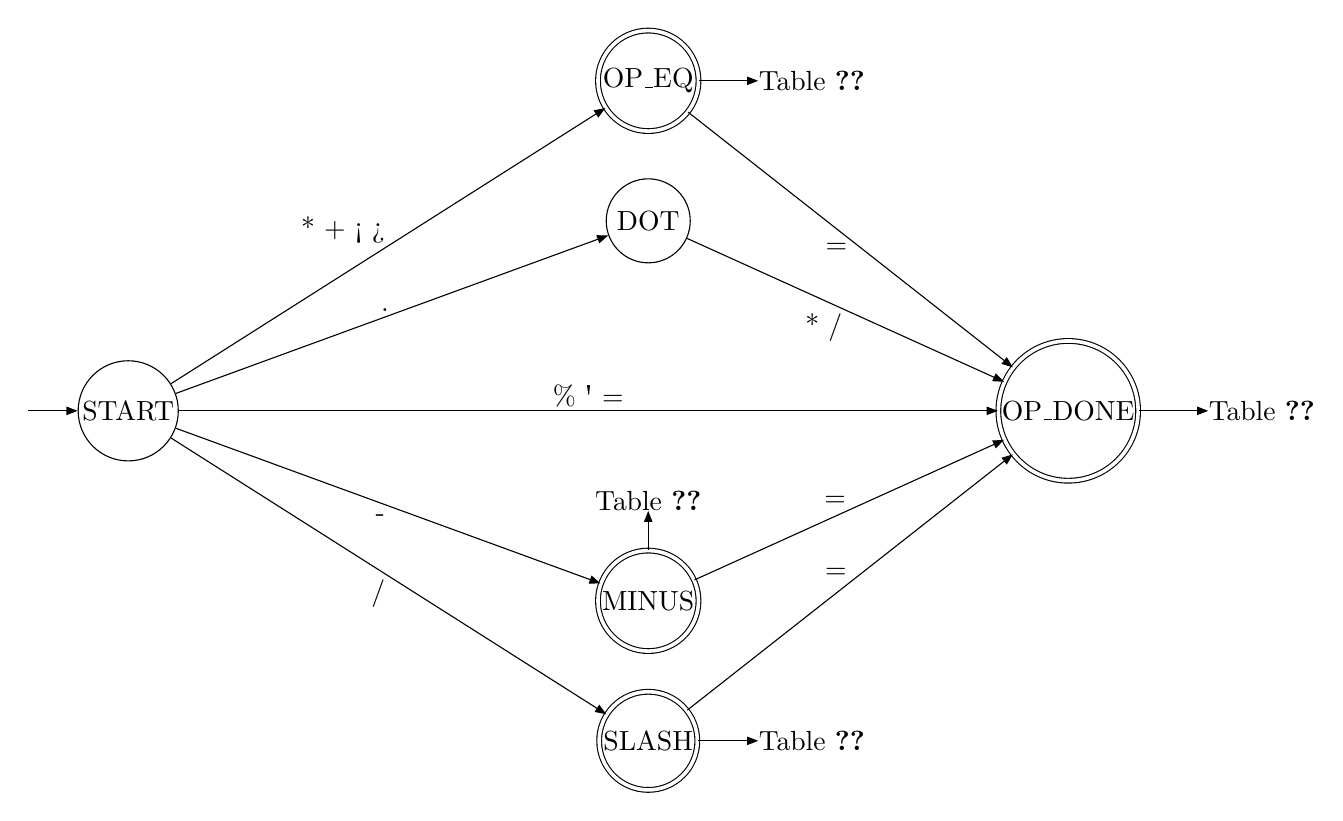
\begin{tikzpicture}[x=1in,y=1in,line width=0.4pt]
\node[draw,circle,fill=white,inner sep=1pt,minimum size=0.42in] (START) at (0.5,4.55) {START};
\node[draw,circle,fill=white,inner sep=1pt,minimum size=0.42in,double,double distance=1.3pt] (OP_DONE) at (5.2,4.55) {OP\_DONE};
\node[draw,circle,fill=white,inner sep=1pt,minimum size=0.42in,double,double distance=1.3pt] (MINUS) at (3.1,3.6) {MINUS};
\node[draw,circle,fill=white,inner sep=1pt,minimum size=0.42in,double,double distance=1.3pt] (OP_EQ) at (3.1,6.2) {OP\_EQ};
\node[draw,circle,fill=white,inner sep=1pt,minimum size=0.42in,double,double distance=1.3pt] (SLASH) at (3.1,2.9) {SLASH};
\node[draw,circle,fill=white,inner sep=1pt,minimum size=0.42in] (DOT) at (3.1,5.5) {DOT};
\draw[-{Triangle[length=4bp,width=3bp]}] (0.0,4.55) -- (START);
\node[inner sep=0pt,align=left,anchor=west] (OP_DONE-out) at (5.9,4.55) {Table~\ref{tab:ops}};
\node[inner sep=0pt,align=left,anchor=south] (MINUS-out) at (3.1,4.05) {Table~\ref{tab:ops}};
\node[inner sep=0pt,align=left,anchor=west] (OP_EQ-out) at (3.65,6.2) {Table~\ref{tab:ops}};
\node[inner sep=0pt,align=left,anchor=west] (SLASH-out) at (3.65,2.9) {Table~\ref{tab:ops}};
\draw[-{Triangle[length=4bp,width=3bp]}] (START) to[bend left=0] node[pos=0.5,above,inner sep=1pt,align=center] {\code{\%} \code{\textquotesingle{}} \code{=}} (OP_DONE);
\draw[-{Triangle[length=4bp,width=3bp]}] (START) to[bend left=0] node[pos=0.5,below left,inner sep=1pt,align=center] {\code{-}} (MINUS);
\draw[-{Triangle[length=4bp,width=3bp]}] (START) to[bend left=0] node[pos=0.5,above left,inner sep=1pt,align=center] {\code{*} \code{+} \code{<} \code{>}} (OP_EQ);
\draw[-{Triangle[length=4bp,width=3bp]}] (START) to[bend left=0] node[pos=0.5,below left,inner sep=1pt,align=center] {\code{/}} (SLASH);
\draw[-{Triangle[length=4bp,width=3bp]}] (START) to[bend left=0] node[pos=0.5,above left,inner sep=1pt,align=center] {\code{.}} (DOT);
\draw[-{Triangle[length=4bp,width=3bp]}] (MINUS) to[bend left=0] node[pos=0.5,above left,inner sep=1pt,align=center] {\code{=}} (OP_DONE);
\draw[-{Triangle[length=4bp,width=3bp]}] (OP_EQ) to[bend left=0] node[pos=0.5,below left,inner sep=1pt,align=center] {\code{=}} (OP_DONE);
\draw[-{Triangle[length=4bp,width=3bp]}] (SLASH) to[bend left=0] node[pos=0.5,above left,inner sep=1pt,align=center] {\code{=}} (OP_DONE);
\draw[-{Triangle[length=4bp,width=3bp]}] (DOT) to[bend left=0] node[pos=0.5,below left,inner sep=1pt,align=center] {\code{*} \code{/}} (OP_DONE);
\draw[-{Triangle[length=4bp,width=3bp]}] (OP_DONE) to[bend left=0] (OP_DONE-out.west);
\draw[-{Triangle[length=4bp,width=3bp]}] (MINUS) to[bend left=0] (MINUS-out.south);
\draw[-{Triangle[length=4bp,width=3bp]}] (OP_EQ) to[bend left=0] (OP_EQ-out.west);
\draw[-{Triangle[length=4bp,width=3bp]}] (SLASH) to[bend left=0] (SLASH-out.west);
\end{tikzpicture}
\end{adjustbox}
\caption{DFA for operators.}
\label{fig:dfa-ops}
\end{figure}

\subsection{Constants}

A constant is a bool constant, an int literal, a float literal or a string
literal.

\begin{itemize}
    \item bool constants: \code{0} \code{1}
    \item int literal: \code{[0-9]+}
    \item float literal: \code{[0-9]+\symbol{92}.[0-9]+} or
    \code{[0-9]+(\symbol{92}.[0-9]+)?[eE][+-]?[0-9]+}
    \item string literal: \code{\symbol{34}[\symbol{94}\symbol{34}\symbol{92}n]*\symbol{34}}
\end{itemize}

Digits are read in \code{INT}. A dot followed by digits leads through
\code{INT\_DOT} to \code{FLOAT}. An \code{e} or \code{E} after \code{INT} or
\code{FLOAT} leads to \code{EXP}, an optional sign to \code{EXP\_SIGN}, and
digits to \code{FLOAT\_EXP}. A quote starts \code{STR\_BODY}, which loops on
every character except a newline or a quote, and the closing quote reaches
\code{STR\_END}. \code{INT}, \code{FLOAT}, \code{FLOAT\_EXP} and
\code{STR\_END} are accepting. The lexer emits \code{0} and \code{1} as int
literals, so the bool constant is never emitted.

\code{INT\_DOT}, \code{EXP}, and \code{EXP\_SIGN} are not accepting, so a
partial literal such as \code{1.} or \code{1e+} is not a number, and the lexer
falls back to the longest number that was complete, as described in
Section~\ref{sec:lexer-algorithm}. A float must have digits on both sides of
the dot, so \code{1.} and \code{.5} are lexical errors. A digit followed by a
letter other than \code{e} or \code{E} has no transition, so \code{12abc} is
read as the integer \code{12} followed by the identifier \code{abc}. There
are no escape sequences in strings, and a string cannot span lines: a newline
inside a string has no transition, so a string that is missing its closing
quote never reaches an accepting state and is reported as an error.

\begin{figure}[H]
\centering
\begin{adjustbox}{max width=\linewidth,max height=0.42\textheight}
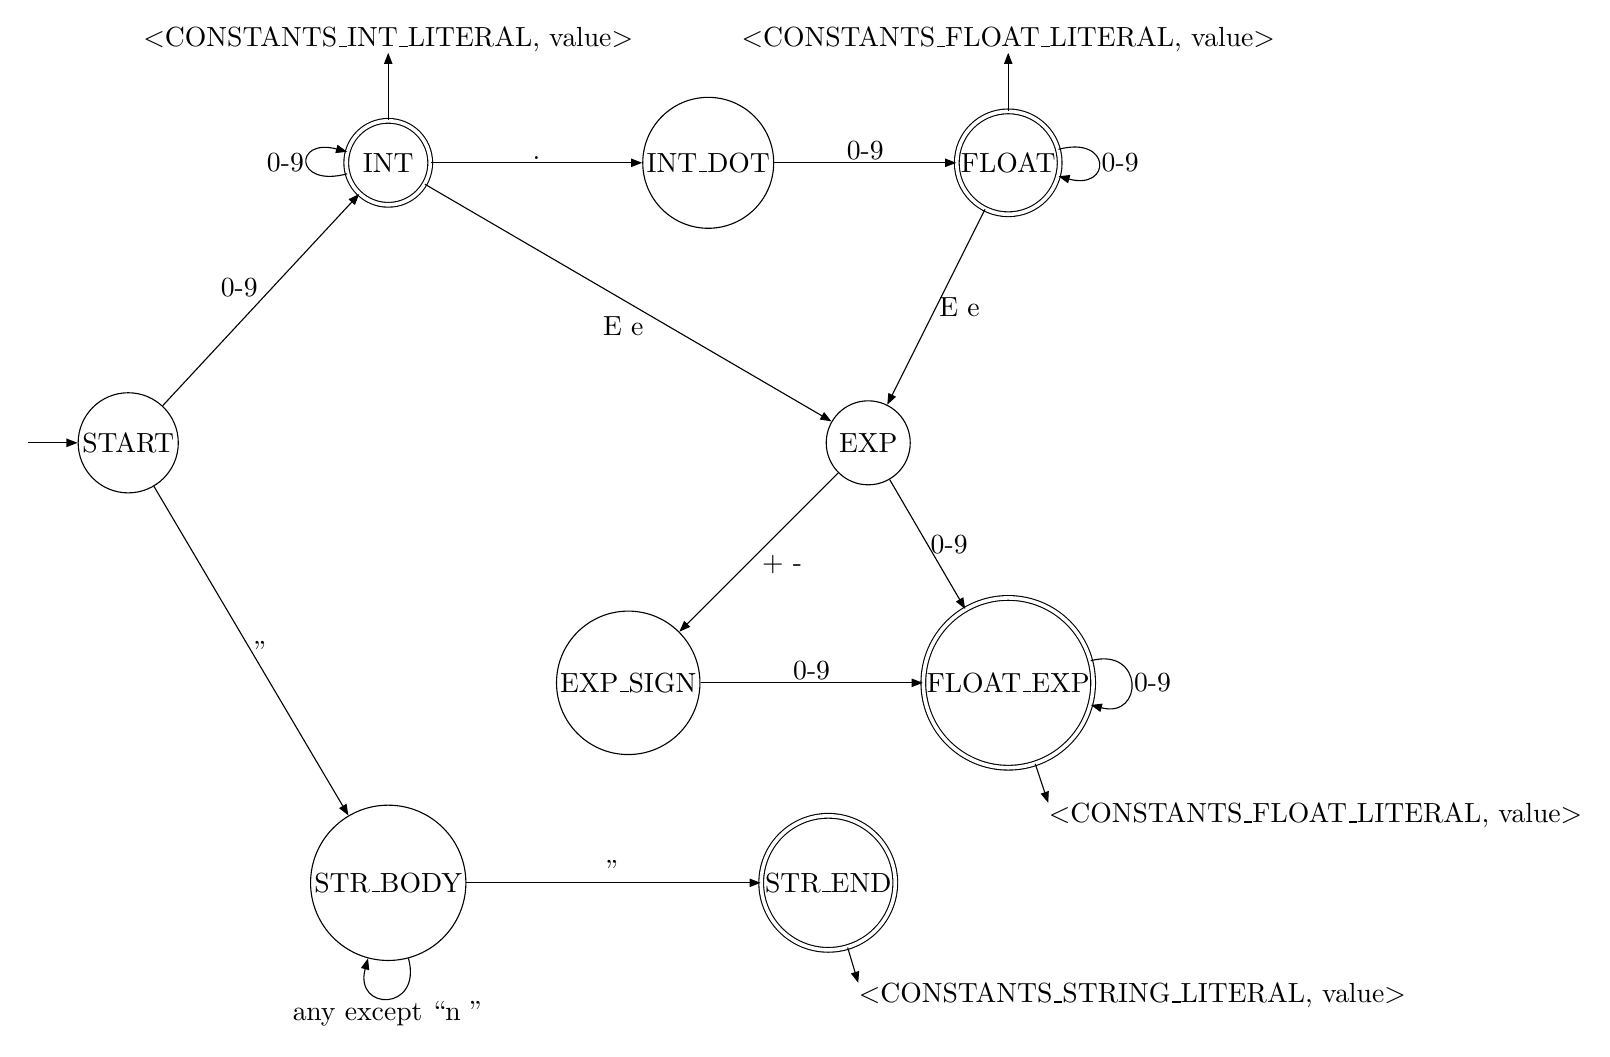
\begin{tikzpicture}[x=1in,y=1in,line width=0.4pt]
\node[draw,circle,fill=white,inner sep=1pt,minimum size=0.42in] (START) at (0.6,3.1) {START};
\node[draw,circle,fill=white,inner sep=1pt,minimum size=0.42in,double,double distance=1.3pt] (INT) at (1.9,4.5) {INT};
\node[draw,circle,fill=white,inner sep=1pt,minimum size=0.42in] (INT_DOT) at (3.5,4.5) {INT\_DOT};
\node[draw,circle,fill=white,inner sep=1pt,minimum size=0.42in,double,double distance=1.3pt] (FLOAT) at (5.0,4.5) {FLOAT};
\node[draw,circle,fill=white,inner sep=1pt,minimum size=0.42in] (EXP) at (4.3,3.1) {EXP};
\node[draw,circle,fill=white,inner sep=1pt,minimum size=0.42in] (EXP_SIGN) at (3.1,1.9) {EXP\_SIGN};
\node[draw,circle,fill=white,inner sep=1pt,minimum size=0.42in,double,double distance=1.3pt] (FLOAT_EXP) at (5.0,1.9) {FLOAT\_EXP};
\node[draw,circle,fill=white,inner sep=1pt,minimum size=0.42in] (STR_BODY) at (1.9,0.9) {STR\_BODY};
\node[draw,circle,fill=white,inner sep=1pt,minimum size=0.42in,double,double distance=1.3pt] (STR_END) at (4.1,0.9) {STR\_END};
\draw[-{Triangle[length=4bp,width=3bp]}] (0.09999999999999998,3.1) -- (START);
\node[inner sep=0pt,align=left,anchor=south] (INT-out) at (1.9,5.05) {\textless{}CONSTANTS\_INT\_LITERAL, value\textgreater{}};
\node[inner sep=0pt,align=left,anchor=south] (FLOAT-out) at (5.0,5.05) {\textless{}CONSTANTS\_FLOAT\_LITERAL, value\textgreater{}};
\node[inner sep=0pt,align=left,anchor=north west] (FLOAT_EXP-out) at (5.2,1.3) {\textless{}CONSTANTS\_FLOAT\_LITERAL, value\textgreater{}};
\node[inner sep=0pt,align=left,anchor=north west] (STR_END-out) at (4.25,0.4) {\textless{}CONSTANTS\_STRING\_LITERAL, value\textgreater{}};
\draw[-{Triangle[length=4bp,width=3bp]}] (START) to[bend left=0] node[pos=0.5,above left,inner sep=1pt,align=center] {\code{0-9}} (INT);
\draw[-{Triangle[length=4bp,width=3bp]}] (START) to[bend left=0] node[pos=0.5,right,inner sep=1pt,align=center] {\code{\symbol{34}}} (STR_BODY);
\path[-{Triangle[length=4bp,width=3bp]}] (INT) edge[loop left,min distance=7mm] node[left,inner sep=1pt,align=center] {\code{0-9}} (INT);
\draw[-{Triangle[length=4bp,width=3bp]}] (INT) to[bend left=0] node[pos=0.5,above,inner sep=1pt,align=center] {\code{.}} (INT_DOT);
\draw[-{Triangle[length=4bp,width=3bp]}] (INT) to[bend left=0] node[pos=0.55,below left,inner sep=1pt,align=center] {\code{E} \code{e}} (EXP);
\draw[-{Triangle[length=4bp,width=3bp]}] (INT_DOT) to[bend left=0] node[pos=0.5,above,inner sep=1pt,align=center] {\code{0-9}} (FLOAT);
\path[-{Triangle[length=4bp,width=3bp]}] (FLOAT) edge[loop right,min distance=7mm] node[right,inner sep=1pt,align=center] {\code{0-9}} (FLOAT);
\draw[-{Triangle[length=4bp,width=3bp]}] (FLOAT) to[bend left=0] node[pos=0.5,right,inner sep=1pt,align=center] {\code{E} \code{e}} (EXP);
\draw[-{Triangle[length=4bp,width=3bp]}] (EXP) to[bend left=0] node[pos=0.5,below right,inner sep=1pt,align=center] {\code{+} \code{-}} (EXP_SIGN);
\draw[-{Triangle[length=4bp,width=3bp]}] (EXP) to[bend left=0] node[pos=0.5,right,inner sep=1pt,align=center] {\code{0-9}} (FLOAT_EXP);
\draw[-{Triangle[length=4bp,width=3bp]}] (EXP_SIGN) to[bend left=0] node[pos=0.5,above,inner sep=1pt,align=center] {\code{0-9}} (FLOAT_EXP);
\path[-{Triangle[length=4bp,width=3bp]}] (FLOAT_EXP) edge[loop right,min distance=7mm] node[right,inner sep=1pt,align=center] {\code{0-9}} (FLOAT_EXP);
\path[-{Triangle[length=4bp,width=3bp]}] (STR_BODY) edge[loop below,min distance=7mm] node[below,inner sep=1pt,align=center] {\code{any except \symbol{92}n \symbol{34}}} (STR_BODY);
\draw[-{Triangle[length=4bp,width=3bp]}] (STR_BODY) to[bend left=0] node[pos=0.5,above,inner sep=1pt,align=center] {\code{\symbol{34}}} (STR_END);
\draw[-{Triangle[length=4bp,width=3bp]}] (INT) to[bend left=0] (INT-out.south);
\draw[-{Triangle[length=4bp,width=3bp]}] (FLOAT) to[bend left=0] (FLOAT-out.south);
\draw[-{Triangle[length=4bp,width=3bp]}] (FLOAT_EXP) to[bend left=0] (FLOAT_EXP-out.north west);
\draw[-{Triangle[length=4bp,width=3bp]}] (STR_END) to[bend left=0] (STR_END-out.north west);
\end{tikzpicture}
\end{adjustbox}
\caption{DFA for constants.}
\label{fig:dfa-const}
\end{figure}

\subsection{Compiler Tokens}

The end of the input emits \textless COMPILER\_EOF,\textgreater. The scanner
checks for the end of the input before it runs the DFA, so the code has no
state for it, and the transition goes straight from the start state to the
token. When the next character has no transition and no accepting state was passed, the DFA is in
\code{DEAD}, the error state of the code, and the text read so far is emitted
as \textless COMPILER\_ERROR,\textgreater.

\begin{figure}[H]
\centering
\begin{adjustbox}{max width=\linewidth,max height=0.25\textheight}
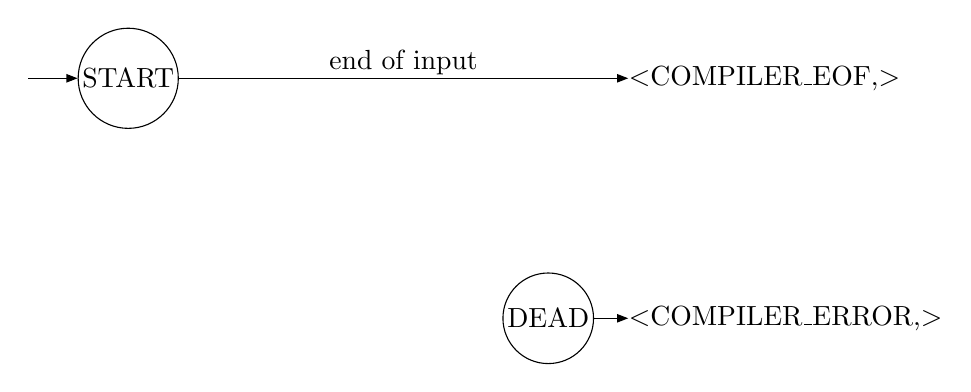
\begin{tikzpicture}[x=1in,y=1in,line width=0.4pt]
\node[draw,circle,fill=white,inner sep=1pt,minimum size=0.42in] (START) at (0.9,1.8) {START};
\node[draw,circle,fill=white,inner sep=1pt,minimum size=0.42in] (DEAD) at (3.0,0.6) {DEAD};
\draw[-{Triangle[length=4bp,width=3bp]}] (0.4,1.8) -- (START);
\node[inner sep=0pt,align=left,anchor=west] (eof-out) at (3.4,1.8) {\textless{}COMPILER\_EOF,\textgreater{}};
\node[inner sep=0pt,align=left,anchor=west] (DEAD-out) at (3.4,0.6) {\textless{}COMPILER\_ERROR,\textgreater{}};
\draw[-{Triangle[length=4bp,width=3bp]}] (START) to[bend left=0] node[pos=0.5,above,inner sep=1pt,align=center] {\code{end of input}} (eof-out.west);
\draw[-{Triangle[length=4bp,width=3bp]}] (DEAD) to[bend left=0] (DEAD-out.west);
\end{tikzpicture}
\end{adjustbox}
\caption{DFA for the compiler tokens.}
\label{fig:dfa-compiler}
\end{figure}

\subsection{Skipped Input}

Skipped input is whitespace and comments. Whitespace is a run of the \code{WS}
and \code{NL} classes and stays in \code{WS}. A comment starts with \code{//}
and runs up to, but not including, the next newline, staying in
\code{COMMENT}. \code{WS} and \code{COMMENT} are accepting but emit no token.
\code{SLASH} is not accepting in this automaton, because a single \code{/} is
not skipped input: it is the division operator of Section~\ref{sec:ops}.

\begin{figure}[H]
\centering
\begin{adjustbox}{max width=\linewidth,max height=0.35\textheight}
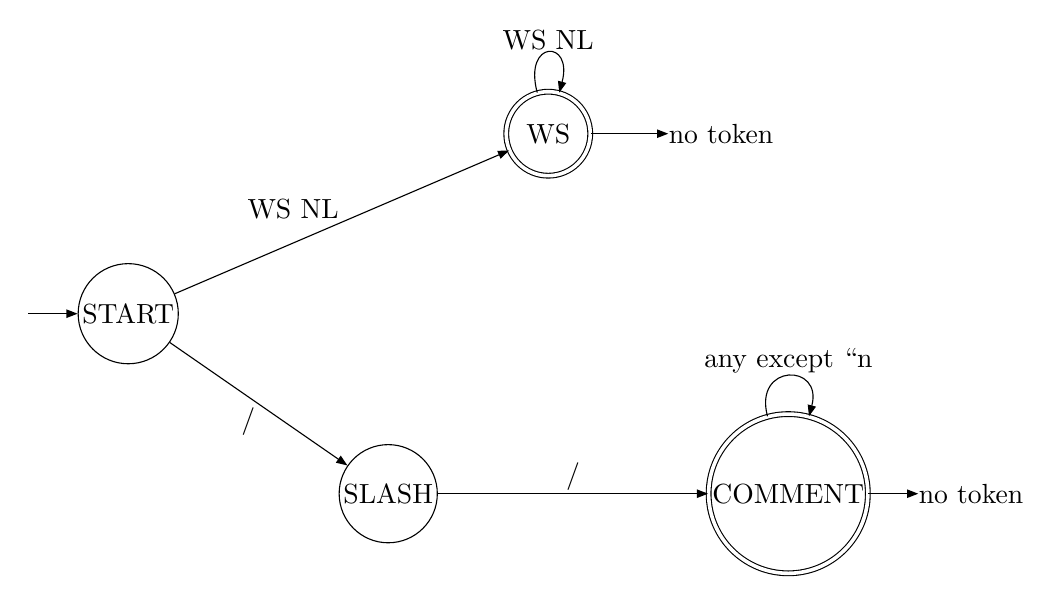
\begin{tikzpicture}[x=1in,y=1in,line width=0.4pt]
\node[draw,circle,fill=white,inner sep=1pt,minimum size=0.42in] (START) at (0.9,1.6) {START};
\node[draw,circle,fill=white,inner sep=1pt,minimum size=0.42in] (SLASH) at (2.2,0.7) {SLASH};
\node[draw,circle,fill=white,inner sep=1pt,minimum size=0.42in,double,double distance=1.3pt] (COMMENT) at (4.2,0.7) {COMMENT};
\node[draw,circle,fill=white,inner sep=1pt,minimum size=0.42in,double,double distance=1.3pt] (WS) at (3.0,2.5) {WS};
\draw[-{Triangle[length=4bp,width=3bp]}] (0.4,1.6) -- (START);
\node[inner sep=0pt,align=left,anchor=west] (COMMENT-out) at (4.85,0.7) {no token};
\node[inner sep=0pt,align=left,anchor=west] (WS-out) at (3.6,2.5) {no token};
\draw[-{Triangle[length=4bp,width=3bp]}] (START) to[bend left=0] node[pos=0.5,below left,inner sep=1pt,align=center] {\code{/}} (SLASH);
\draw[-{Triangle[length=4bp,width=3bp]}] (START) to[bend left=0] node[pos=0.5,above left,inner sep=1pt,align=center] {\code{WS} \code{NL}} (WS);
\draw[-{Triangle[length=4bp,width=3bp]}] (SLASH) to[bend left=0] node[pos=0.5,above,inner sep=1pt,align=center] {\code{/}} (COMMENT);
\path[-{Triangle[length=4bp,width=3bp]}] (COMMENT) edge[loop above,min distance=7mm] node[above,inner sep=1pt,align=center] {\code{any except \symbol{92}n}} (COMMENT);
\path[-{Triangle[length=4bp,width=3bp]}] (WS) edge[loop above,min distance=7mm] node[above,inner sep=1pt,align=center] {\code{WS} \code{NL}} (WS);
\draw[-{Triangle[length=4bp,width=3bp]}] (COMMENT) to[bend left=0] (COMMENT-out.west);
\draw[-{Triangle[length=4bp,width=3bp]}] (WS) to[bend left=0] (WS-out.west);
\end{tikzpicture}
\end{adjustbox}
\caption{DFA for whitespace and comments.}
\label{fig:dfa-skip}
\end{figure}

\subsection{The Merged DFA}

The classes are merged into one DFA, the one the lexer runs. Its states carry the
names the source gives them.

\begin{enumerate}
    \item A new start state has a transition for the first character of
    every class.
    \item Classes that share a prefix share states. Keywords, type names
    and identifiers are all read in IDENT, and operators and punctuation
    end in OP\_DONE, MINUS, OP\_EQ, SLASH, DOT and DOT\_DOT.
    \item A state that is accepting for one class stays accepting in the
    merged DFA, so MINUS and SLASH are accepting here.
    \item IDENT emits \textless IDENTIFIER, value\textgreater, which
    Table~\ref{tab:lookup} replaces when the lexeme is a keyword or type
    name. OP\_EQ and OP\_DONE emit different tokens depending on the
    lexeme. The arrow from each of them names the tables that list them.
    \item The DFA runs until the next character has no transition. The
    token of the last accepting state passed is emitted, and if none was
    passed the consumed text is a \textless COMPILER\_ERROR,\textgreater{}
    token. DEAD is not drawn: every missing transition leads to it.
\end{enumerate}

\begin{figure}[H]
\centering
\begin{adjustbox}{max width=\linewidth,max height=0.85\textheight}
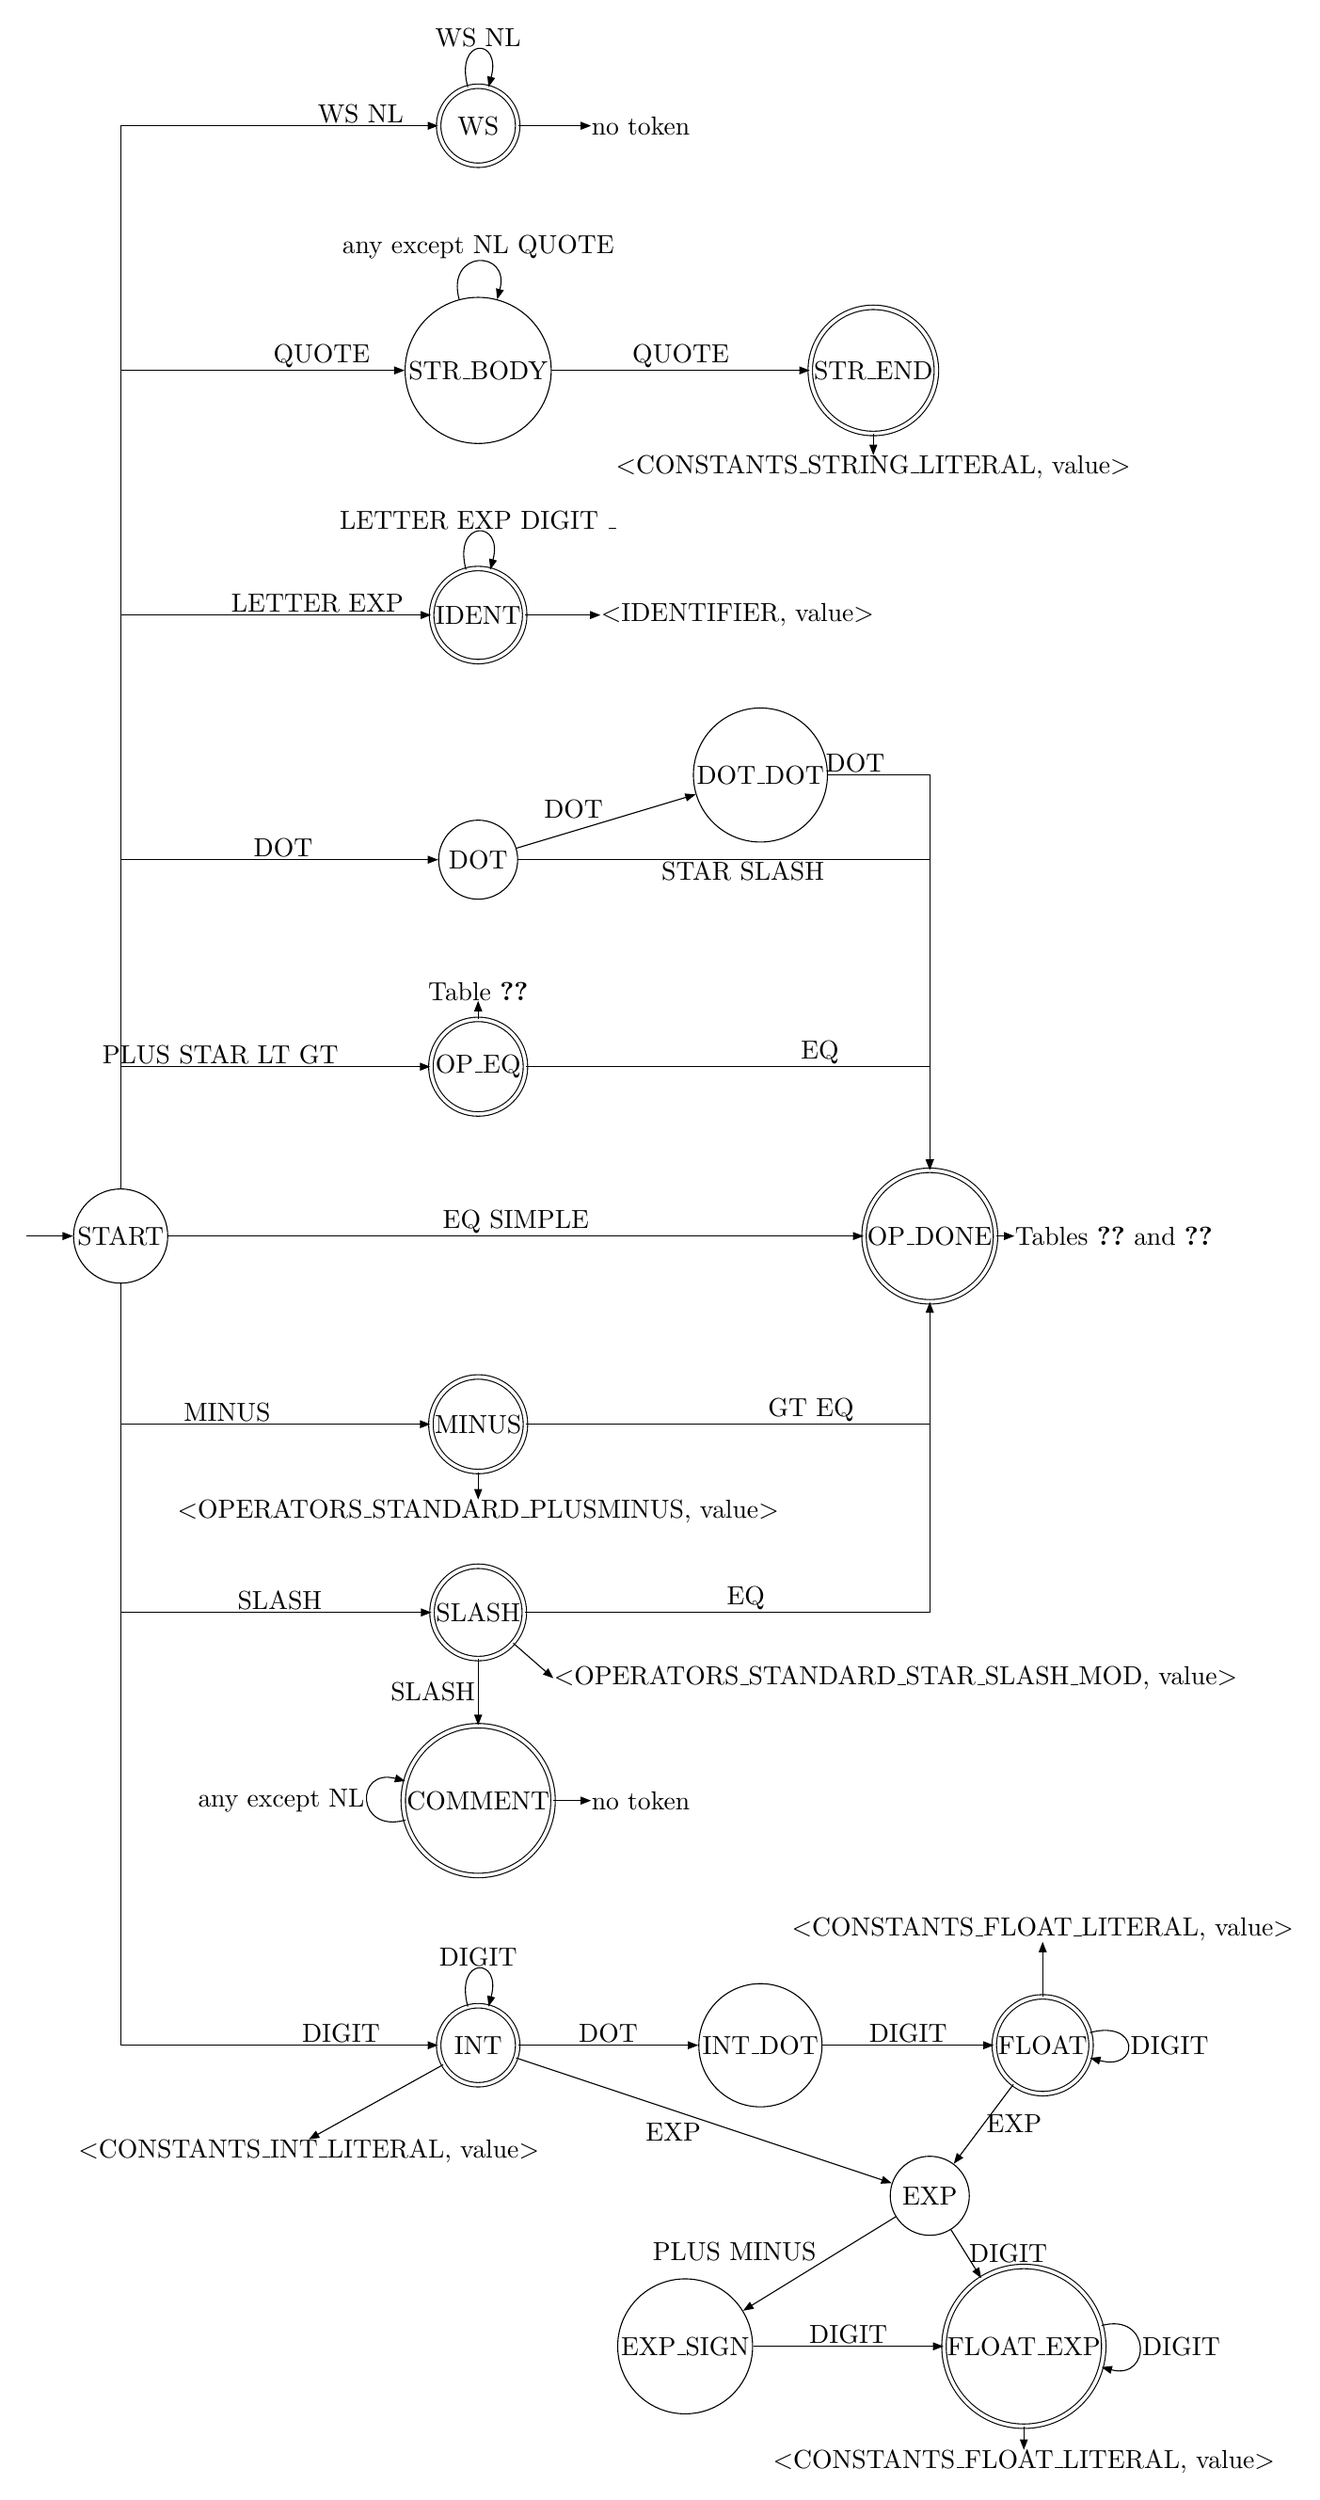
\begin{tikzpicture}[x=1in,y=1in,line width=0.4pt]
\node[draw,circle,fill=white,inner sep=1pt,minimum size=0.42in] (START) at (0.6,7.1) {START};
\node[draw,circle,fill=white,inner sep=1pt,minimum size=0.42in,double,double distance=1.3pt] (IDENT) at (2.5,10.4) {IDENT};
\node[draw,circle,fill=white,inner sep=1pt,minimum size=0.42in,double,double distance=1.3pt] (INT) at (2.5,2.8) {INT};
\node[draw,circle,fill=white,inner sep=1pt,minimum size=0.42in] (INT_DOT) at (4.0,2.8) {INT\_DOT};
\node[draw,circle,fill=white,inner sep=1pt,minimum size=0.42in,double,double distance=1.3pt] (FLOAT) at (5.5,2.8) {FLOAT};
\node[draw,circle,fill=white,inner sep=1pt,minimum size=0.42in] (EXP) at (4.9,2.0) {EXP};
\node[draw,circle,fill=white,inner sep=1pt,minimum size=0.42in] (EXP_SIGN) at (3.6,1.2000000000000002) {EXP\_SIGN};
\node[draw,circle,fill=white,inner sep=1pt,minimum size=0.42in,double,double distance=1.3pt] (FLOAT_EXP) at (5.4,1.2000000000000002) {FLOAT\_EXP};
\node[draw,circle,fill=white,inner sep=1pt,minimum size=0.42in,double,double distance=1.3pt] (OP_DONE) at (4.9,7.1) {OP\_DONE};
\node[draw,circle,fill=white,inner sep=1pt,minimum size=0.42in,double,double distance=1.3pt] (MINUS) at (2.5,6.1) {MINUS};
\node[draw,circle,fill=white,inner sep=1pt,minimum size=0.42in,double,double distance=1.3pt] (OP_EQ) at (2.5,8.0) {OP\_EQ};
\node[draw,circle,fill=white,inner sep=1pt,minimum size=0.42in,double,double distance=1.3pt] (SLASH) at (2.5,5.1) {SLASH};
\node[draw,circle,fill=white,inner sep=1pt,minimum size=0.42in,double,double distance=1.3pt] (COMMENT) at (2.5,4.1) {COMMENT};
\node[draw,circle,fill=white,inner sep=1pt,minimum size=0.42in] (DOT) at (2.5,9.100000000000001) {DOT};
\node[draw,circle,fill=white,inner sep=1pt,minimum size=0.42in] (DOT_DOT) at (4.0,9.55) {DOT\_DOT};
\node[draw,circle,fill=white,inner sep=1pt,minimum size=0.42in] (STR_BODY) at (2.5,11.700000000000001) {STR\_BODY};
\node[draw,circle,fill=white,inner sep=1pt,minimum size=0.42in,double,double distance=1.3pt] (STR_END) at (4.6,11.700000000000001) {STR\_END};
\node[draw,circle,fill=white,inner sep=1pt,minimum size=0.42in,double,double distance=1.3pt] (WS) at (2.5,13.0) {WS};
\draw[-{Triangle[length=4bp,width=3bp]}] (0.09999999999999998,7.1) -- (START);
\node[inner sep=0pt,align=left,anchor=west] (IDENT-out) at (3.15,10.4) {\textless{}IDENTIFIER, value\textgreater{}};
\node[inner sep=0pt,align=left,anchor=north] (INT-out) at (1.6,2.3) {\textless{}CONSTANTS\_INT\_LITERAL, value\textgreater{}};
\node[inner sep=0pt,align=left,anchor=south] (FLOAT-out) at (5.5,3.3499999999999996) {\textless{}CONSTANTS\_FLOAT\_LITERAL, value\textgreater{}};
\node[inner sep=0pt,align=left,anchor=north] (FLOAT_EXP-out) at (5.4,0.65) {\textless{}CONSTANTS\_FLOAT\_LITERAL, value\textgreater{}};
\node[inner sep=0pt,align=left,anchor=west] (OP_DONE-out) at (5.35,7.1) {Tables~\ref{tab:punct} and~\ref{tab:ops}};
\node[inner sep=0pt,align=left,anchor=north] (MINUS-out) at (2.5,5.7) {\textless{}OPERATORS\_STANDARD\_PLUSMINUS, value\textgreater{}};
\node[inner sep=0pt,align=left,anchor=south] (OP_EQ-out) at (2.5,8.35) {Table~\ref{tab:ops}};
\node[inner sep=0pt,align=left,anchor=west] (SLASH-out) at (2.9,4.75) {\textless{}OPERATORS\_STANDARD\_STAR\_SLASH\_MOD, value\textgreater{}};
\node[inner sep=0pt,align=left,anchor=west] (COMMENT-out) at (3.1,4.1) {no token};
\node[inner sep=0pt,align=left,anchor=north] (STR_END-out) at (4.6,11.25) {\textless{}CONSTANTS\_STRING\_LITERAL, value\textgreater{}};
\node[inner sep=0pt,align=left,anchor=west] (WS-out) at (3.1,13.0) {no token};
\draw[-{Triangle[length=4bp,width=3bp]}] (IDENT) to[bend left=0] (IDENT-out.west);
\draw[-{Triangle[length=4bp,width=3bp]}] (INT) to[bend left=0] (INT-out.north);
\draw[-{Triangle[length=4bp,width=3bp]}] (FLOAT) to[bend left=0] (FLOAT-out.south);
\draw[-{Triangle[length=4bp,width=3bp]}] (FLOAT_EXP) to[bend left=0] (FLOAT_EXP-out.north);
\draw[-{Triangle[length=4bp,width=3bp]}] (OP_DONE) to[bend left=0] (OP_DONE-out.west);
\draw[-{Triangle[length=4bp,width=3bp]}] (MINUS) to[bend left=0] (MINUS-out.north);
\draw[-{Triangle[length=4bp,width=3bp]}] (OP_EQ) to[bend left=0] (OP_EQ-out.south);
\draw[-{Triangle[length=4bp,width=3bp]}] (SLASH) to[bend left=0] (SLASH-out.west);
\draw[-{Triangle[length=4bp,width=3bp]}] (COMMENT) to[bend left=0] (COMMENT-out.west);
\draw[-{Triangle[length=4bp,width=3bp]}] (STR_END) to[bend left=0] (STR_END-out.north);
\draw[-{Triangle[length=4bp,width=3bp]}] (WS) to[bend left=0] (WS-out.west);
\draw[-{Triangle[length=4bp,width=3bp]}] (START) |- node[pos=0.817,above,inner sep=1pt,align=center] {\code{LETTER} \code{EXP}} (IDENT);
\draw[-{Triangle[length=4bp,width=3bp]}] (START) |- node[pos=0.847,above,inner sep=1pt,align=center] {\code{DIGIT}} (INT);
\draw[-{Triangle[length=4bp,width=3bp]}] (START) to[bend left=0] node[pos=0.5,above,inner sep=1pt,align=center] {\code{EQ} \code{SIMPLE}} (OP_DONE);
\draw[-{Triangle[length=4bp,width=3bp]}] (START) |- node[pos=0.672,above,inner sep=1pt,align=center] {\code{MINUS}} (MINUS);
\draw[-{Triangle[length=4bp,width=3bp]}] (START) |- node[pos=0.661,above,inner sep=1pt,align=center] {\code{PLUS} \code{STAR} \code{LT} \code{GT}} (OP_EQ);
\draw[-{Triangle[length=4bp,width=3bp]}] (START) |- node[pos=0.756,above,inner sep=1pt,align=center] {\code{SLASH}} (SLASH);
\draw[-{Triangle[length=4bp,width=3bp]}] (START) |- node[pos=0.756,above,inner sep=1pt,align=center] {\code{DOT}} (DOT);
\draw[-{Triangle[length=4bp,width=3bp]}] (START) |- node[pos=0.854,above,inner sep=1pt,align=center] {\code{QUOTE}} (STR_BODY);
\draw[-{Triangle[length=4bp,width=3bp]}] (START) |- node[pos=0.878,above,inner sep=1pt,align=center] {\code{WS} \code{NL}} (WS);
\path[-{Triangle[length=4bp,width=3bp]}] (IDENT) edge[loop above,min distance=7mm] node[above,inner sep=1pt,align=center] {\code{LETTER} \code{EXP} \code{DIGIT} \code{\_}} (IDENT);
\path[-{Triangle[length=4bp,width=3bp]}] (INT) edge[loop above,min distance=7mm] node[above,inner sep=1pt,align=center] {\code{DIGIT}} (INT);
\draw[-{Triangle[length=4bp,width=3bp]}] (INT) to[bend left=0] node[pos=0.5,above,inner sep=1pt,align=center] {\code{DOT}} (INT_DOT);
\draw[-{Triangle[length=4bp,width=3bp]}] (INT) to[bend left=0] node[pos=0.5,below left,inner sep=1pt,align=center] {\code{EXP}} (EXP);
\draw[-{Triangle[length=4bp,width=3bp]}] (INT_DOT) to[bend left=0] node[pos=0.5,above,inner sep=1pt,align=center] {\code{DIGIT}} (FLOAT);
\path[-{Triangle[length=4bp,width=3bp]}] (FLOAT) edge[loop right,min distance=7mm] node[right,inner sep=1pt,align=center] {\code{DIGIT}} (FLOAT);
\draw[-{Triangle[length=4bp,width=3bp]}] (FLOAT) to[bend left=0] node[pos=0.5,right,inner sep=1pt,align=center] {\code{EXP}} (EXP);
\draw[-{Triangle[length=4bp,width=3bp]}] (EXP) to[bend left=0] node[pos=0.5,above left,inner sep=1pt,align=center] {\code{PLUS} \code{MINUS}} (EXP_SIGN);
\draw[-{Triangle[length=4bp,width=3bp]}] (EXP) to[bend left=0] node[pos=0.5,right,inner sep=1pt,align=center] {\code{DIGIT}} (FLOAT_EXP);
\draw[-{Triangle[length=4bp,width=3bp]}] (EXP_SIGN) to[bend left=0] node[pos=0.5,above,inner sep=1pt,align=center] {\code{DIGIT}} (FLOAT_EXP);
\path[-{Triangle[length=4bp,width=3bp]}] (FLOAT_EXP) edge[loop right,min distance=7mm] node[right,inner sep=1pt,align=center] {\code{DIGIT}} (FLOAT_EXP);
\draw[-{Triangle[length=4bp,width=3bp]}] (MINUS) -| node[pos=0.353,above,inner sep=1pt,align=center] {\code{GT} \code{EQ}} (OP_DONE);
\draw[-{Triangle[length=4bp,width=3bp]}] (OP_EQ) -| node[pos=0.364,above,inner sep=1pt,align=center] {\code{EQ}} (OP_DONE);
\draw[-{Triangle[length=4bp,width=3bp]}] (SLASH) -| node[pos=0.273,above,inner sep=1pt,align=center] {\code{EQ}} (OP_DONE);
\draw[-{Triangle[length=4bp,width=3bp]}] (SLASH) to[bend left=0] node[pos=0.5,left,inner sep=1pt,align=center] {\code{SLASH}} (COMMENT);
\path[-{Triangle[length=4bp,width=3bp]}] (COMMENT) edge[loop left,min distance=7mm] node[left,inner sep=1pt,align=center] {\code{any except NL}} (COMMENT);
\draw[-{Triangle[length=4bp,width=3bp]}] (DOT) -| node[pos=0.273,below,inner sep=1pt,align=center] {\code{STAR} \code{SLASH}} (OP_DONE);
\draw[-{Triangle[length=4bp,width=3bp]}] (DOT) to[bend left=0] node[pos=0.5,above left,inner sep=1pt,align=center] {\code{DOT}} (DOT_DOT);
\draw[-{Triangle[length=4bp,width=3bp]}] (DOT_DOT) -| node[pos=0.134,above,inner sep=1pt,align=center] {\code{DOT}} (OP_DONE);
\path[-{Triangle[length=4bp,width=3bp]}] (STR_BODY) edge[loop above,min distance=7mm] node[above,inner sep=1pt,align=center] {\code{any except NL QUOTE}} (STR_BODY);
\draw[-{Triangle[length=4bp,width=3bp]}] (STR_BODY) to[bend left=0] node[pos=0.5,above,inner sep=1pt,align=center] {\code{QUOTE}} (STR_END);
\path[-{Triangle[length=4bp,width=3bp]}] (WS) edge[loop above,min distance=7mm] node[above,inner sep=1pt,align=center] {\code{WS} \code{NL}} (WS);
\end{tikzpicture}
\end{adjustbox}
\caption{The merged DFA of the lexer.}
\label{fig:dfa-merged}
\end{figure}

\section{The Lexical Analyzer Algorithm}
\label{sec:lexer-algorithm}

The scanner exposes a single operation, \code{next}, which returns the next
token each time it is called. It keeps the source text, the current position,
and the current line and column, both counted from 1. The reference
implementation is a C++ program.

\subsection{Maximal Munch}

Each call to \code{next} starts at the current position and walks the
transition table for as long as a transition exists. Whenever it enters an
accepting state it records that state and the position reached. When it
reaches the dead state, or the end of the input, it rewinds to the last
recorded position. This is the longest match rule: the lexer always takes the
longest prefix that forms a token \cite{aho2006compilers}. The rewinding is
what allows one automaton to handle lexemes that share a prefix.

The text \code{0...2} shows this. The lexer reads \code{0}, which is accepting,
and then a dot, which moves to \code{INT\_DOT}. The next dot has no transition
from \code{INT\_DOT}, so the lexer rewinds to the \code{0} and emits it as an
integer literal. Scanning resumes at the first dot, which reaches
\code{OP\_DONE} after three dots and emits the ellipsis, and then \code{2} is
scanned on its own. In the same way, \code{1e+;} is scanned as the integer
\code{1}, the identifier \code{e}, and the operator \code{+}, because
\code{EXP} and \code{EXP\_SIGN} are not accepting.

\subsection{The Scanning Loop}

Listing~\ref{lst:scan-loop} shows the body of \code{next}. The character class
mapping is written \code{classOf}, and \code{advance} moves the position
forward while updating the line and column. The two lookup tables described
earlier are used through two functions. The function \code{lookupKeyword}
handles words, and \code{lookupOperator} handles operators.

\begin{lstlisting}[style=pseudocode, float=tbp,
    caption={The scanning loop of the lexer.}, label=lst:scan-loop]
function next():
    loop:
        if pos >= length(src):
            return Token(COMPILER_EOF)

        start <- pos
        state <- START
        lastAccept <- DEAD
        lastEnd <- start
        cur <- start

        while cur < length(src):
            nxt <- TRANSITION[state][classOf(src[cur])]
            if nxt is DEAD: break
            state <- nxt
            cur <- cur + 1
            if ACTION[state] is not NONE:
                lastAccept <- state
                lastEnd <- cur

        if lastAccept is DEAD:
            end <- start + 1 if cur = start else cur
            lexeme <- src[start .. end)
            advance(end - start)
            return Token(COMPILER_ERROR, lexeme)

        lexeme <- src[start .. lastEnd)
        advance(lastEnd - start)

        switch ACTION[lastAccept]:
            WORD:    type <- lookupKeyword(lexeme)
            INT:     type <- CONSTANTS_INT_LITERAL
            FLOAT:   type <- CONSTANTS_FLOAT_LITERAL
            OP:      type <- lookupOperator(lexeme)
            STRING:  type <- CONSTANTS_STRING_LITERAL
            SKIP:    continue    // scan again
        return Token(type, lexeme)
\end{lstlisting}

Each token also records the line and column where it started, which are taken
before the position moves.

\subsection{Resolving the Token}

The action of the last accepting state says how to name the lexeme. A word is
looked up in the keyword table, which also holds the type names, and falls back
to an identifier. An operator or punctuator is looked up in the operator
table. Integer literals, float literals, and string literals are named
directly by their state. Whitespace and comments are skipped, and the loop
starts again from the new position, so \code{next} never returns them.

The token set lists a bool constant token for the values \code{0} and
\code{1}. The lexer does not produce it. Both values are scanned as integer
literals, and interpreting them as booleans is left to the parser.

\subsection{Errors}

If the walk never reached an accepting state, the text it consumed becomes the
lexeme of an error token, and at least one character is consumed so that
scanning always makes progress. The lexer then reports the lexeme on the
standard error stream together with its line and column, and scanning
resumes right after it. One run therefore reports every lexical error in a
file. Table~\ref{tab:lexer-errors} shows how some invalid inputs are reported.

\begin{table}[tbp]
\centering
\small
\renewcommand{\arraystretch}{1.1}
\begin{tabular}{@{}ll@{}}
\toprule
\textbf{Input} & \textbf{Reported lexeme} \\
\midrule
\code{\_hidden} & \code{\_} \\
\code{1.} & \code{.} \\
\code{.5} & \code{.} \\
\code{1.5.2} & \code{.} \\
\code{3..4} & \code{..} \\
\code{"unterminated} & \code{"unterminated} \\
\code{!=} & \code{!} \\
\code{a @ b} & \code{@} \\
\bottomrule
\end{tabular}
\caption{Examples of lexical errors.}
\label{tab:lexer-errors}
\end{table}

\subsection{Token Output}

The lexer writes one token per line in the form \code{<TYPE, value>}, ending
with the end of file token. Only some tokens have a value part: identifiers,
scalar type names, integer, float, and string literals, the arithmetic
operators, and the assignment operators. These are the tokens whose Values
column is filled in Table~\ref{tab:token-set}. Every other token is written
with an empty value part, for example \code{<PUNCTUATION\_LBRACE,>}.

\subsection{Sample Runs}

To see the algorithm at work, we run the lexer on three statements. For each
lexeme, the tables list the states the automaton visits, starting from
\code{START}, followed by the lookup that names the lexeme when there is one,
and ending in the token that comes out. The whitespace between lexemes
takes the automaton through \code{WS}, which is skipped, so it does not appear
in the tables. After the last lexeme of the input, the lexer returns the end of
file token, \code{<COMPILER\_EOF,>}, which is also left out.

\medskip
\noindent\begin{minipage}{\textwidth}
\noindent\textbf{Statement 1.} The first statement declares a variable. Every lexeme is either a word, a number, or a single character.

\begin{lstlisting}
i32 count = 10;
\end{lstlisting}

\begin{center}
\footnotesize
\renewcommand{\arraystretch}{1.1}
\setlength{\tabcolsep}{4pt}
\begin{tabular}{@{}l>{\raggedright\arraybackslash}p{370pt}@{}}
\toprule
\textbf{Lexeme} & \textbf{States visited, lookup, and token} \\
\midrule
\code{i32} & \tok{START} $\to$ \tok{IDENT} $\to$ \tok{IDENT} $\to$ \tok{IDENT} $\to$ lookup(keyword table) $\to$ \tok{<DT_SCALAR, i32>} \\
\code{count} & \tok{START} $\to$ \tok{IDENT} $\to$ \tok{IDENT} $\to$ \tok{IDENT} $\to$ \tok{IDENT} $\to$ \tok{IDENT} $\to$ lookup(keyword table) $\to$ \tok{<IDENTIFIER, count>} \\
\code{=} & \tok{START} $\to$ \tok{OP_DONE} $\to$ lookup(operator table) $\to$ \tok{<OPERATORS_ASSIGNMENT, =>} \\
\code{10} & \tok{START} $\to$ \tok{INT} $\to$ \tok{INT} $\to$ \tok{<CONSTANTS_INT_LITERAL, 10>} \\
\code{;} & \tok{START} $\to$ \tok{OP_DONE} $\to$ lookup(operator table) $\to$ \tok{<PUNCTUATION_SEMICOLON,>} \\
\bottomrule
\end{tabular}
\end{center}
\end{minipage}
\medskip


\medskip
\noindent\begin{minipage}{\textwidth}
\noindent\textbf{Statement 2.} The second statement has a float with an exponent, and a matrix operator that is written without spaces around it.

\begin{lstlisting}
f32 y = 2.5e-3 + a.*b;
\end{lstlisting}

\begin{center}
\footnotesize
\renewcommand{\arraystretch}{1.1}
\setlength{\tabcolsep}{4pt}
\begin{tabular}{@{}l>{\raggedright\arraybackslash}p{370pt}@{}}
\toprule
\textbf{Lexeme} & \textbf{States visited, lookup, and token} \\
\midrule
\code{f32} & \tok{START} $\to$ \tok{IDENT} $\to$ \tok{IDENT} $\to$ \tok{IDENT} $\to$ lookup(keyword table) $\to$ \tok{<DT_SCALAR, f32>} \\
\code{y} & \tok{START} $\to$ \tok{IDENT} $\to$ lookup(keyword table) $\to$ \tok{<IDENTIFIER, y>} \\
\code{=} & \tok{START} $\to$ \tok{OP_DONE} $\to$ lookup(operator table) $\to$ \tok{<OPERATORS_ASSIGNMENT, =>} \\
\code{2.5e-3} & \tok{START} $\to$ \tok{INT} $\to$ \tok{INT_DOT} $\to$ \tok{FLOAT} $\to$ \tok{EXP} $\to$ \tok{EXP_SIGN} $\to$ \tok{FLOAT_EXP} $\to$ \tok{<CONSTANTS_FLOAT_LITERAL, 2.5e-3>} \\
\code{+} & \tok{START} $\to$ \tok{OP_EQ} $\to$ lookup(operator table) $\to$ \tok{<OPERATORS_STANDARD_PLUSMINUS, +>} \\
\code{a} & \tok{START} $\to$ \tok{IDENT} $\to$ lookup(keyword table) $\to$ \tok{<IDENTIFIER, a>} \\
\code{.*} & \tok{START} $\to$ \tok{DOT} $\to$ \tok{OP_DONE} $\to$ lookup(operator table) $\to$ \tok{<OPERATORS_MATRIX_DOT_STAR,>} \\
\code{b} & \tok{START} $\to$ \tok{IDENT} $\to$ lookup(keyword table) $\to$ \tok{<IDENTIFIER, b>} \\
\code{;} & \tok{START} $\to$ \tok{OP_DONE} $\to$ lookup(operator table) $\to$ \tok{<PUNCTUATION_SEMICOLON,>} \\
\bottomrule
\end{tabular}
\end{center}
\end{minipage}
\medskip


\medskip
\noindent\begin{minipage}{\textwidth}
\noindent\textbf{Statement 3.} The third statement is the range loop, and the range \code{1...5} is the case where the lexer has to rewind.

\begin{lstlisting}
for (i32 i = 1...5) {
\end{lstlisting}

\begin{center}
\footnotesize
\renewcommand{\arraystretch}{1.1}
\setlength{\tabcolsep}{4pt}
\begin{tabular}{@{}l>{\raggedright\arraybackslash}p{370pt}@{}}
\toprule
\textbf{Lexeme} & \textbf{States visited, lookup, and token} \\
\midrule
\code{for} & \tok{START} $\to$ \tok{IDENT} $\to$ \tok{IDENT} $\to$ \tok{IDENT} $\to$ lookup(keyword table) $\to$ \tok{<KW_LOOPS_FOR,>} \\
\code{(} & \tok{START} $\to$ \tok{OP_DONE} $\to$ lookup(operator table) $\to$ \tok{<PUNCTUATION_LPAREN,>} \\
\code{i32} & \tok{START} $\to$ \tok{IDENT} $\to$ \tok{IDENT} $\to$ \tok{IDENT} $\to$ lookup(keyword table) $\to$ \tok{<DT_SCALAR, i32>} \\
\code{i} & \tok{START} $\to$ \tok{IDENT} $\to$ lookup(keyword table) $\to$ \tok{<IDENTIFIER, i>} \\
\code{=} & \tok{START} $\to$ \tok{OP_DONE} $\to$ lookup(operator table) $\to$ \tok{<OPERATORS_ASSIGNMENT, =>} \\
\code{1} & \tok{START} $\to$ \tok{INT} $\to$ \tok{INT_DOT} \textit{(no move on the next dot, rewind to \tok{INT})} $\to$ \tok{<CONSTANTS_INT_LITERAL, 1>} \\
\code{...} & \tok{START} $\to$ \tok{DOT} $\to$ \tok{DOT_DOT} $\to$ \tok{OP_DONE} $\to$ lookup(operator table) $\to$ \tok{<PUNCTUATION_ELLIPSIS,>} \\
\code{5} & \tok{START} $\to$ \tok{INT} $\to$ \tok{<CONSTANTS_INT_LITERAL, 5>} \\
\code{)} & \tok{START} $\to$ \tok{OP_DONE} $\to$ lookup(operator table) $\to$ \tok{<PUNCTUATION_RPAREN,>} \\
\code{\{} & \tok{START} $\to$ \tok{OP_DONE} $\to$ lookup(operator table) $\to$ \tok{<PUNCTUATION_LBRACE,>} \\
\bottomrule
\end{tabular}
\end{center}
\end{minipage}
\medskip


\medskip
\noindent In the first two runs, every lexeme is accepted at the last state it reaches,
and the lexer never has to go back. The word \code{i32} ends in \code{IDENT},
and the keyword table turns it into a type token. The float \code{2.5e-3} is
the longest path in the automaton, and it passes through three states that
are not accepting. In the third run, the \code{1} is followed by a dot, which
moves the automaton to \code{INT\_DOT}. The next character is another dot, which
has no transition there, so the lexer goes back to the last accepting state,
which was reached after the \code{1}, and returns the integer. The scan for the
next token then starts at the first dot, and reads all three of them.

\section{Lexers in the Real World}
\label{sec:lexers-real-world}

The lexer of OctaC is deliberately small. This section looks at how lexers
are built in practice, what they handle that ours does not, and which
simplifications we made.

\subsection{Lexer Generators}

Many lexers are produced by a generator such as Lex \cite{lesk1975lex} or its
successor Flex \cite{flex-manual}. The programmer writes a list of regular
expressions, each with an action. The generator converts them into a
deterministic finite automaton and emits a table-driven scanner
\cite{aho2006compilers}. Two rules resolve conflicts between patterns: the
longest match wins, and among patterns that match the same length, the one
listed first wins \cite{lesk1975lex,flex-manual}. Our scanner follows the
longest match rule. The second rule is not needed, because keywords are not
patterns of their own.

Flex recommends matching identifiers with one pattern and looking keywords up
in a table, instead of writing a pattern for each keyword
\cite{flex-manual}, which is what OctaC does. Flex also warns that a scanner
which has to back up over several characters is slower, and offers ways to
find and remove such cases \cite{flex-manual}. Our scanner backs up too, as the
run of \code{1...5} shows, but only over a few characters. Generators also
compress their tables \cite{aho2006compilers}. Ours has 19 states and 17
character classes, which is small enough to be stored as it is.

\subsection{Hand-Written Lexers}

Many production compilers do not use a generator. The lexer of the GNU C
preprocessor is coded by hand and is not implemented as a state machine
\cite{gcc-cppinternals}, and Clang has a hand-written lexer that scans the
source buffer directly \cite{clang-internals}. A hand-written lexer gives full
control over the speed of the scanner, the quality of error messages, and the
handling of features that regular expressions describe poorly. The lexer of
OctaC sits between the two approaches. The table is written by hand, but the
scanning loop is the same one that a generator would emit.

\subsection{What Real Lexers Handle}

Lexers for established languages deal with many things that OctaC leaves out:

\begin{itemize}
    \item \textbf{Richer literals.} Numbers may be written in hexadecimal,
    octal, or binary, with digit separators and type suffixes. Strings have
    escape sequences, raw forms, and may span lines \cite{rust-reference}.
    \item \textbf{More kinds of comments.} Block comments exist in many
    languages, and in Rust they can be nested \cite{rust-reference}.
    \item \textbf{Unicode.} Identifiers may contain letters from any script,
    following the rules of Unicode Standard Annex 31
    \cite{unicode-uax31,python-reference}.
    \item \textbf{Layout.} Python's lexer produces indent and dedent tokens
    from the indentation of each line \cite{python-reference}. The lexer of
    Go inserts semicolons at the ends of lines by a fixed rule, so programs
    can leave most of them out \cite{go-spec}.
    \item \textbf{Preprocessing.} A C lexer works together with the
    preprocessor, which handles macros and file inclusion
    \cite{gcc-cppinternals}.
\end{itemize}

\subsection{Simplifications in OctaC}

Table~\ref{tab:lexer-simplifications} summarizes the differences. Each of the
simplifications keeps the automaton small, and each could be lifted later by
adding states and character classes to the table.

\begin{table}[tbp]
\centering
\small
\renewcommand{\arraystretch}{1.15}
\begin{tabular}{@{}>{\raggedright\arraybackslash}p{62pt}>{\raggedright\arraybackslash}p{190pt}>{\raggedright\arraybackslash}p{180pt}@{}}
\toprule
\textbf{Concern} & \textbf{Real-world lexers} & \textbf{OctaC} \\
\midrule
Construction & Generated from regular expressions, or written by hand \cite{flex-manual,clang-internals} & One hand-written transition table \\
Characters & Unicode text, usually as UTF-8 & Bytes; anything outside the listed classes is an error \\
Identifiers & Unicode letters allowed \cite{unicode-uax31} & ASCII letters, digits, and underscores, starting with a letter \\
Numbers & Hexadecimal, binary, separators, suffixes \cite{rust-reference} & Decimal integers and floats, with an optional exponent \\
Strings & Escapes, raw strings, multiple lines \cite{rust-reference} & None of these: one line, no escapes \\
Comments & Block comments, sometimes nested \cite{rust-reference} & Line comments with \code{//} only \\
Layout & Indentation tokens, semicolon insertion \cite{python-reference,go-spec} & Whitespace is not significant, and semicolons are explicit \\
Preprocessing & Macros and file inclusion \cite{gcc-cppinternals} & None \\
Keywords & Table lookup after matching an identifier \cite{flex-manual} & Same \\
Errors & Diagnostics with recovery & Error token, a diagnostic, and scanning resumes \\
Input & Streamed through a buffer & The whole file is read into memory \\
\bottomrule
\end{tabular}
\caption{Real-world lexers compared with the OctaC lexer.}
\label{tab:lexer-simplifications}
\end{table}


% Future chapters are added here as the language and compiler develop.
% \input{chp03-grammar}
% \input{chp04-parser}
% \input{chp05-semantic-analysis}
% \input{chp06-code-generation}

\chapter*{Conclusion}

Conclusion will be updated once the project is complete....
\addcontentsline{toc}{chapter}{Conclusion}

{
% The following prevents latex from splitting a bibliography entry with a page
% break
\interlinepenalty=10000
% Since we're using natbib in numbers mode, we don't need plainnat,
% which exists to feed authors and years back in to natbib.  As a
% result, it complains about entries without years, which we don't
% care about.
%\bibliographystyle{plainnat}
\bibliographystyle{plain}
\nocite{*}
\bibliography{bibliography}
\addcontentsline{toc}{chapter}{Bibliography}
}

\printindex

\end{document}